%%%%%%%%%%%%%%%%%%%%%%%%%%%%%%%%%%%%%%%%%%%%%%%%%%%%%%%
%% Bachelor's & Master's Thesis Template             %%
%% Copyleft by Artur M. Brodzki & Piotr Woźniak      %%
%% Faculty of Electronics and Information Technology %%
%% Warsaw University of Technology, 2019-2020        %%
%%%%%%%%%%%%%%%%%%%%%%%%%%%%%%%%%%%%%%%%%%%%%%%%%%%%%%%

\documentclass[
    left=2.5cm,         % Sadly, generic margin parameter
    right=2.5cm,        % doesnt't work, as it is
    top=2.5cm,          % superseded by more specific
    bottom=3cm,         % left...bottom parameters.
    bindingoffset=6mm,  % Optional binding offset.
    nohyphenation=false % You may turn off hyphenation, if don't like.
]{template/eiti-thesis}
\usepackage{cleveref}

\addbibresource{ref.bib} % Plik .bib z bibliografią

\begin{document}

%--------------------------------------
% Strona tytułowa
%--------------------------------------
\instytut{Telekomunikacji}
\kierunek{Cyberbezpieczeństwo}
\title{Wybrane metody przeprowadzania i detekcji OSINT}
\engtitle{Selected methods of conducting and detecting OSINT}
\author{tulski}
\album{304217}
\promotor{dr inż. Mariusz Sepczuk}
\date{\the\year}
\maketitle

%--------------------------------------
% Streszczenie po polsku
%--------------------------------------
\newpage %\cleardoublepage % Zaczynamy od nieparzystej strony
\streszczenie \todo{ \lipsum[1] }
\slowakluczowe XXX, XXX, XXX

%--------------------------------------
% Streszczenie po angielsku
%--------------------------------------
\newpage
\abstract \todo{ \lipsum[1] }
\keywords XXX, XXX, XXX

%--------------------------------------
% Oświadczenie o autorstwie
%--------------------------------------
\newpage %\cleardoublepage  % Zaczynamy od nieparzystej strony
\makeauthorship

%--------------------------------------
% Spis treści
%--------------------------------------
\newpage %\cleardoublepage % Zaczynamy od nieparzystej strony

\section*{\contentsname}

\startcontents[mainsections]
\printcontents[mainsections]{l}{1}{\setcounter{tocdepth}{3}}

%--------------------------------------
% Rozdziały
%--------------------------------------
%\cleardoublepage % Zaczynamy od nieparzystej strony
\pagestyle{headings}
\newpage

\section{Teoria związana z tematem pracy}\label{sec:teoria}

\subsection{OSINT}\label{subsec:osint}

\todo{OSINT}

\subsection{Scraping}\label{subsec:scraping}

\todo{Scraping}

\subsection{Web Scraping}\label{subsec:web-scraping}

\todo{Web Scraping}
\newpage


\section{Przegląd metod detekcji web scrapingu}\label{sec:przeglad-rozwiazan}

\subsection{Rate Limiting}\label{subsec:rate-limiting}

Rate Limiting to technika kontrolująca tempo, w jakim klienci mogą wysyłać żądania do serwera API\@.
W tym celu zlicza się liczbę żądań w określonym przedziale czasowym, a następnie ustala, czy ich częstotliwość nie przekracza maksymalnego dopuszczalnego progu~\cite{api-rate-limit-adoption}.

Rozwiązanie zazwyczaj polega na kalkulacji czasu między każdym żądaniem z każdego adresu IP\@.
W przypadku, kiedy liczba żądań z danego adresu IP przekroczy ustalony limit w danym oknie czasowym, żądanie kończy się odpowiednim błędem.
W tym przypadku adres IP służy jako identyfikator klienta~\cite{cloudflare-what-is-rate-limiting}.
Nie jest to jednak jedyne rozwiązanie, jako że dopuszcza się również identyfikatory innego rodzaju.

Brak rate limitingu API jest, według \emph{OWASP API Security Top 10}, uznawany za podatność.
W punkcie \emph{API4:2019 Lack of Resources \& Rate Limiting}, autorzy wskazują, że:\@
\begin{displayquote}[\citetitle*{owasp-api-security-top-10}~\cite{owasp-api-security-top-10}, tłum. własne]
    ``Żądania API zużywają zasoby takie jak sieć, CPU, pamięć i miejsce na dysku.
    Ilość zasobów potrzebnych do zaspokojenia żądania w dużej mierze zależy od danych wejściowych użytkownika i logiki biznesowej koncówki.
    Należy również wziąć pod uwagę fakt, że żądania od wielu klientów API konkurują o te same zasoby.
    API jest podatne na problemy, jeśli brakuje przynajmniej jednego z następujących limitów lub są one ustawione nieodpowiednio (np.\ zbyt niskie/wysokie):
    \begin{itemize}
        \item limit czasu wykonania,
        \item maksymalna alokowana pamięć,
        \item liczba deskryptorów plików,
        \item liczba procesów,
        \item rozmiar ładunku żądania (np.\ przesyłane pliki),
        \item liczba żądań na klienta/zasób,
        \item liczba rekordów na stronę zwracanych w pojedynczej odpowiedzi na żądanie.''
    \end{itemize}
\end{displayquote}

Rate Limiting stosuje się do ochrony ograniczonych zasobów, obrony przed atakami typu odmowa dostępu (ang. \emph{DoS, Denial of Service})
oraz blokowania aktywności botów generujących duże nadużycia\@.
Scrapery, będąc automatycznym oprogramowaniem, często kreują dużą liczbę zapytań w krótkim czasie, znacznie większą niż człowiek podczas standardowego korzystania z serwisu.
Istotne jest zatem takie skonfigurowanie reguł rate limitingu, aby znaleźć swoisty złoty środek, pozwalający na zablokowanie zautomatyzowanego pobierania danych bez jednoczesnego ograniczania dostępu prawdziwym użytkownikom.

\newpage

\subsection{Reverse Proxy --- blokowanie oparte na regułach}\label{subsec:reverse-proxy}

Termin proxy, w dziedzinie sieci komputerowych, określa aplikacje serwerową, która działa jako pośrednik między klientem wysyłającym żądanie a serwerem docelowym.
Wyróżnia się dwa główne typy proxy: forward proxy i reverse proxy.
Oba z nich działają na brzegu sieci.
W uproszczeniu, pierwszy z nich pośredniczy między klientem a internetem, podczas gdy drugi zarządza ruchem przychodzącym z internetu do serwerów.
Uszczegóławiając, reverse proxy najczęściej znajduje się na brzegu sieci przed jednym lub wieloma serwerami.
Klient wysyła żądanie do serwera proxy, a ten je przechwytuje i przekazuje do serwerów docelowych~\cite{cloudflare-what-is-reverse-proxy}.
Działanie reverse proxy zostało przedstawione na \autoref{fig:reverse-proxy}.

\begin{figure}[H]
    \centering
    \captionsetup{width=.7\linewidth}
    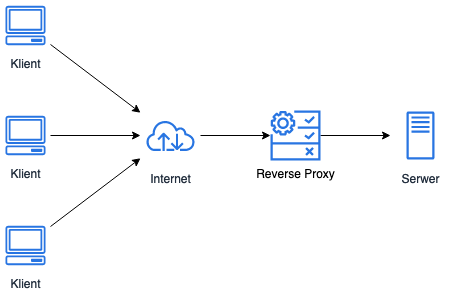
\includegraphics[width=0.8\textwidth]{img/reverse-proxy}
    \caption{Uproszczony schemat działania reverse proxy}
    \label{fig:reverse-proxy}
\end{figure}

Serwery reverse proxy znajdują swoje zastosowanie w detekcji web scrapingu ze względu na swoją zdolność do filtrowania ruchu przychodzącego.
Jak wskazano w \autoref{subsec:scraper}, ruch sieciowy generowany przez scrapery odznacza się niejednokrotnie charakterystycznymi cechami.
Na podstawie każdego z punktów w wspomnianym \autoref{subsec:scraper} można stworzyć regułę blokującą web scraping.

\newpage

\subsection{Browser Fingerprinting}\label{subsec:browser-fingerprinting}

Browser Fingerprint --- odcisk przeglądarki --- to zestaw informacji związanych z środowiskiem przeglądarki internetowej użytkownika, od fizycznego sprzętu, poprzez system operacyjny, aż do oprogramowania i jego konfiguracji~\cite{browser-fingerprinting-a-survey}.
Browser Fingerprinting to proces zbierania i analizy informacji tworzących odcisk przeglądarki.
Proces ten wykorzystuje się w celu identyfikacji i śledzenia użytkowników.
Dąż się do zgromadzenia możliwie wielu rekordów, które połączone razem tworzą unikalną kombinację jednoznacznie identyfikującą użytkownika~\cite{fingerprint-browser-fingerprinting}.
Informacje te najczęściej pochodzą z nagłówków HTTP oraz skryptów uruchamianych bezpośrednio w kontekście przeglądarki internetowej użytkownika.
Zebrane informacje mogą zawierać m.in.:
\begin{itemize}
    \item specyfikacje sprzętową: wersja urządzenia, rozdzielczość ekranu, poziom baterii, pamięć urządzenia, informacje nt. procesora (CPU) i karty graficznej (GPU),
    \item informacje o systemie operacyjnym i przeglądarce: typ i wersja systemu operacyjnego, typ i wersja przeglądarki internetowej, wtyczki zainstalowane w przeglądarce internetowej, obecność blokera reklam, wykorzystywany układ klawiatury, ustawienia przeglądarki (preferowany język, opcje śledzenia, wspieranie ciasteczek), ustawienia systemowe (strefa czasowa, zainstalowane czcionki), parametry WebGL (Web Graphics Library)
    \item informacje sieciowe: adres IP, szczegóły sesji TSL~\cite{browser-fingerprinting-a-survey,zitadel-browser-fingerprinting,zenrows-browser-fingerprinting,fingerprint-browser-fingerprinting}.
\end{itemize}
\noindent Przykładowy odcisk przeglądarki został przedstawiony w \autoref{tab:http-js-attributes}.

Browser Fingerprinting znajduje zastosowanie jako metoda detekcji web scrapingu.
Poprzez zbieranie odcisku przeglądarki i tworzeniu dla niego identyfikatora, możemy wymagać jego podania, tym samym blokując API web scraping.
Istnieją określone elementy odcisku sugerujące użycie metod automatyzacji~\cite{zenrows-browser-fingerprinting}.
Przykładowo, przeglądarki uruchomione przez biblioteki opisywane w \autoref{subsubsec:browser-scraping-theory} charakteryzują się:
ekranem o rozdzielczości 0x0 (Headless Browser),
WebGL z dostawcą \texttt{Brian Paul} lub \texttt{Mesa OffScreen} (Headless Chrome),
User-Agentem zawierającym \texttt{"PhantomJS"}, \texttt{"Headless"}, \texttt{"Electron"} lub \texttt{"slimerjs"},
brakiem zainstalowanych wtyczek, brakiem wspieranych kodeków wideo itd.
Ponadto, scrapery często są uruchomione w chmurach obliczeniowych bez urządzeń peryferyjnych lub środowiska graficznego.

\begin{table}[p]
    \small
    \centering
    \begin{tabular}{|p{0.35\linewidth} | p{0.6\linewidth}|}
        \hline
        \textbf{Atrybut}             & \textbf{Wartość}                                                                                                                                                                                                                                                                                                                                                                                                                              \\ \hline
        User Agent                   & Mozilla/5.0 (Macintosh; Intel Mac OS X 10.15; rv:122.0) Gecko/20100101 Firefox/122.0                                                                                                                                                                                                                                                                                                                                                          \\ \hline
        Platforma                    & MacIntel                                                                                                                                                                                                                                                                                                                                                                                                                                      \\ \hline
        Strefa czasowa               & UTC+01:00 (-60)                                                                                                                                                                                                                                                                                                                                                                                                                               \\ \hline
        Język                        & en-US,en,pl                                                                                                                                                                                                                                                                                                                                                                                                                                   \\ \hline
        Szczegóły ekranu             & szerokość: 1680, wysokość: 1050, depth: 24, dostępna wysokość: 1050, dostępna szerokość: 1680 i inne                                                                                                                                                                                                                                                                                                                                          \\ \hline
        Canvas                       & 
\includegraphics[width=0.9\linewidth]{img/fingerprint-cavas}                                                                                                                                                                                                                                                                                                                                                                                  \\ \hline
        Dostawca WebGL               & Apple                                                                                                                                                                                                                                                                                                                                                                                                                                         \\ \hline
        Renderujący WebGL            & Apple M1                                                                                                                                                                                                                                                                                                                                                                                                                                      \\ \hline
        Dane WebGL                   & 
\includegraphics[width=0.6\linewidth]{img/fingerprint-webgl}                                                                                                                                                                                                                                                                                                                                                                                  \\ \hline
        Parametry WebGL              & Wykryto 26 różnych rozszerzeń.\ Przeanalizowano 25 różnych parametrów ogólnych i 36 różnych precyzji shaderów.                                                                                                                                                                                                                                                                                                                                \\ \hline
        Lista fontów (JS)            & Al Bayan, Al Nile, Al Tarikh, American Typewriter, Andale Mono i 181 innych                                                                                                                                                                                                                                                                                                                                                                   \\ \hline
        Wtyczki &
        --- PDF Viewer; Portable Document Format; internal-pdf-viewer\newline
        --- Chrome PDF Viewer; Portable Document Format; internal-pdf-viewer.\newline
        oraz 3 inne \\ \hline
        Wykorzystanie AdBlock        & Tak                                                                                                                                                                                                                                                                                                                                                                                                                                           \\ \hline
        Do Not Track                 & Tak                                                                                                                                                                                                                                                                                                                                                                                                                                           \\ \hline
        Atrybuty Navigator           & Wykryto 45 obiektów                                                                                                                                                                                                                                                                                                                                                                                                                           \\ \hline
        Urządzenia multimedialne     & 2 wejścia audio, 1 wejście video                                                                                                                                                                                                                                                                                                                                                                                                              \\ \hline
        Kontekst audio               & częstotliwość próbkowania: 48000, stan: wstrzymano                                                                                                                                                                                                                                                                                                                                                                                            \\ \hline
        Wspierane rozszerzenia audio & audio/aac : możliwe, audio/flac : możliwe, audio/mpeg : możliwe, audio/ogg; codecs=\("\)flac\("\)  : prawdopodobnie, audio/ogg; codecs=\("\)vorbis\("\) : prawdopodobnie, audio/ogg; codecs=\("\)opus\("\) : prawdopodobnie, audio/wav; codecs=\("\)1\("\) : prawdopodobnie, audio/webm; codecs=\("\)vorbis\("\) : prawdopodobnie, audio/webm; codecs=\("\)opus\("\) : prawdopodobnie, audio/mp4; codecs=\("\)mp4a\_40\_2\("\) : prawdopodobnie \\ \hline
        Wspierane rozszerzenia video & video/mp4; codecs=\("\)flac\("\) : prawdopodobnie, video/ogg; codecs=\("\)theora\("\) : prawdopodobnie, video/ogg; codecs=\("\)opus\("\) : prawdopodobnie, video/webm; codecs=\("\)vp9, opus\("\) : prawdopodobnie, video/webm; codecs=\("\)vp8, vorbis\("\) : prawdopodobnie,                                                                                                                                                                \\ \hline
        Dostępne elementy            & Location Bar, Menu Bar, Personal Bar, Status Bar, Tool Bar, Local Storage, Session Storage, IndexedDB, Ciasteczka                                                                                                                                                                                                                                                                                                                             \\ \hline
    \end{tabular}
    \caption{Wybrane atrybuty odcisku przeglądarki autora pracy\\Tabela powstała przy pomocy serwisu AM I UNIQUE?\\(\url{https://amiunique.org/})}
    \label{tab:http-js-attributes}
\end{table}

%\begin{enumerate}
%    \item specyfikacje sprzętową:
%    \begin{itemize}
%        \item wersja urządzenia,
%        \item rozdzielczość ekranu,
%        \item poziom baterii,
%        \item pamięć urządzenia,
%        \item informacje nt. procesora (CPU),
%        \item informacje nt. karty graficznej (GPU),
%    \end{itemize}
%    \item informacje o systemie operacyjnym i przeglądarce:
%    \begin{itemize}
%        \item typ i wersja systemu operacyjnego,
%        \item typ i wersja przeglądarki internetowej,
%        \item wtyczki zainstalowane w przeglądarce internetowej (w tym obecność blokera reklam),
%        \item wykorzystywany układ klawiatury,
%        \item ustawienia przeglądarki (preferowany język, opcje śledzenia, wspieranie ciasteczek),
%        \item ustawienia systemowe (strefa czasowa, zainstalowane czcionki),
%        \item parametry WebGL (Web Graphics Library)
%    \end{itemize}
%    \item informacje sieciowe:
%    \begin{itemize}
%        \item adres IP,
%        \item szczegóły sesji TSL~\cite{browser-fingerprinting-a-survey,zitadel-browser-fingerprinting,zenrows-browser-fingerprinting,fingerprint-browser-fingerprinting}.
%    \end{itemize}
%\end{enumerate}

\newpage

\section{Wykorzystane narzędzia}\label{sec:wykorzystane-narzedzia}

\todo{Ten rodział jest o narzędziach - o czym innym miałby być?}

\subsection{Docker}\label{subsec:docker}

Docker \todo{to narzędzie do... konteneryzacji?}
Opisywana w pracy platforma wykorzystuje technologię konteneryzacji oferowaną przez Docker.

\subsection{Kubernetes}\label{subsec:kubernetes}

\todo{Kubernetes to narzędzie do...}

\subsection{Helm}\label{subsec:helm}

Helm to narzędzie będące menadżerem pakietów w środowisku Kubernetes.
Narzędzie znacznie ułatwia proces wdrażania i utrzymywania aplikacji, szczególnie jeśli są one skomplikowane i złożone z kilku elementów.

\subsection{MicroK8s}\label{subsec:microk8s}

Kubernetes stał się niejako standardem w branży IT\@.
Wraz z wzrostem jego popularności, kolejne osoby oraz firmy zaczęły dostosowywać oryginalny projekt do swoich potrzeb, tym samym tworząc jego własne dystrybucje.
Chociaż wszystkie te dystrybucje mają wspólny fundament, jakim jest oryginalny projekt Kubernetes, każda z nich wnosi unikalne funkcje, narzędzia i optymalizacje.
Przykładowo, dystrybucje takie jak Amazon Elastic Kubernetes Service (Amazon EKS), Google Kubernetes Engine (GKE) czy Azure Kubernetes Service (AKS) zostały specjalnie dostosowane pod specyficzne środowisko chmury poszczególnych dostawcy.

Niniejsza praca wykorzystuje dystrybucję MicroK8s\cite{microk8s-docs-home} ze względu na:
\begin{enumerate}
    \item łatwość instalacji i uruchomienia,
    \item fakt, że jest to lekka dystrybucja K8s, co przekłada się na mniejsze wymagania sprzętowe oraz mniejsze zużycie zasobów,
    \item stabilność - dystrybucja jest przygotowania do produkcyjnego uruchomienia,
    \item prostotę zarządzania - MicroK8s udostępnia rozbudowany interfejs wiersza poleceń (ang. \emph{command line interface, CLI}) ułatwiający konfigurację i utrzymanie środowiska.
\end{enumerate}

\subsection{Medusa}\label{subsec:medusa}

Handel, w tym ten internetowy, jest obecny w naszym życiu od dekad.
Przez swoją bogatą historię stał się jedną z najlepiej opisanych i najbardziej dojrzałych domen.
Większość wyzwań i problemów, które mogą się pojawić przy implementacji sklepu internetowego zostało już świetnie udokumentowanych, chociażby w książkach z archetypami (pierwowzorami projektowymi).
W obliczu tego, obecnie niewiele sklepów internetowych jest tworzone od zera, bez podparcia gotowymi rozwiązaniami.

Część praktyczna niniejszej pracy korzysta z rozbudowanego ekosystemu Medusa\cite{medusajs-homepage}.
Wykorzystanie tego typu rozwiązania znacząco przyśpieszyło proces wdrożenia platformy i pozwoliło skupić się na elementach specyficznych dla tematu pracy.
Modularna architektura \emph{Software Development Kit (SDK)} projektu Medusa zawiera moduły dla każdej niezbędnej funkcji sklepu internetowego, chociażby moduł odpowiedzialny za obsługę katalogu produktów, logistykę czy płatności.

\newpage

\section{Projekt i wykonanie platformy}\label{sec:projekt-platformy}

Niniejszy rozdział poświęcony jest platformie sklepu internetowego tulski.com.
Przedmiotem analizy są zarówno komponenty aplikacyjne, jak i infrastrukturalne, które razem tworzą kompletny system e-commerce.

Jak przedstawiono na rysunku~\ref{fig:platform-model}, platforma zawiera moduły do monitoringu, zarządzania certyfikatami, repozytorium obrazów kontenerów, oraz przestrzeń \url{store}, która obejmuje bazę danych, backend, panel administratora oraz witrynę internetową.

Szczegółowy opis i konfiguracja poszczególnych komponentów została przedstawiona w dalszej części rozdziału.

\begin{figure}[p]
    \centering
    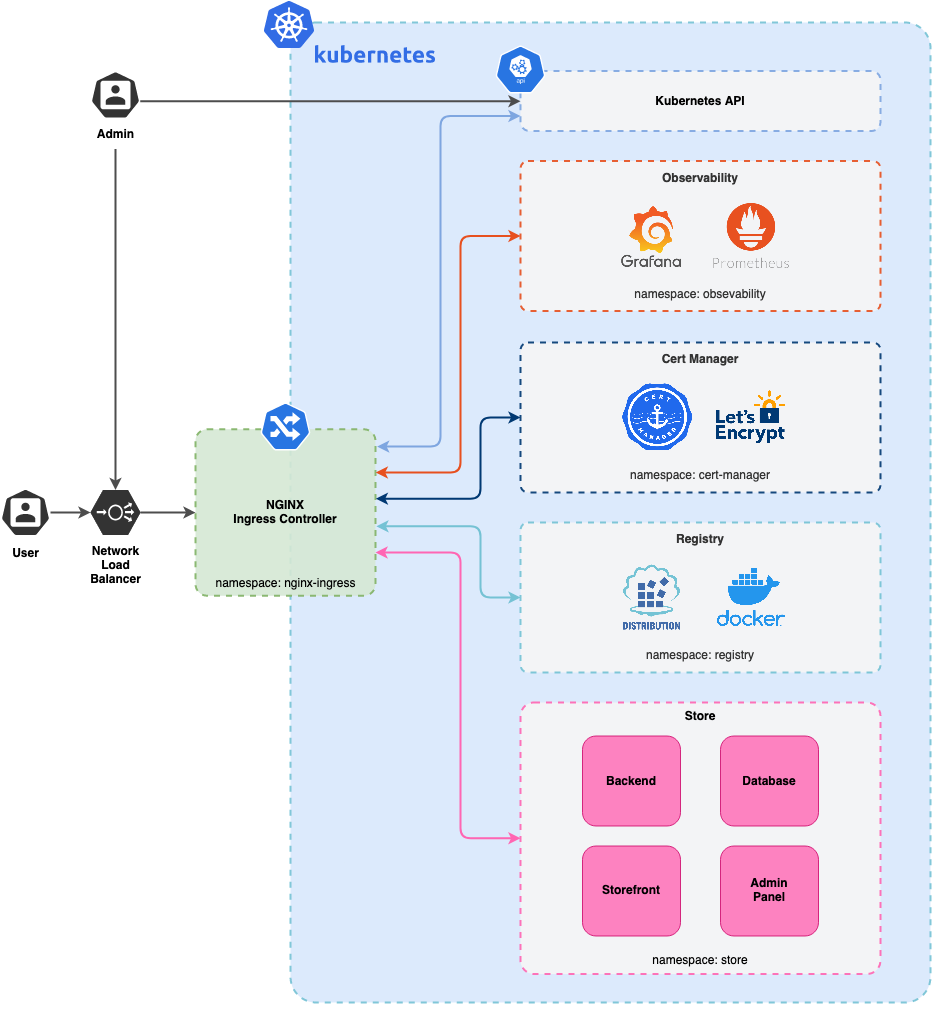
\includegraphics[width=\textwidth]{img/main-infra-model}
    \caption{Model platformy sklepu internetowego tulski}
    \label{fig:platform-model}
\end{figure}

\subsection{Platforma wdrożeniowa}\label{subsec:platforma-wdrozeniowa-kubernetes}

Platformą wdrożeniową dla projektu jest infrastruktura w postaci klastra Kubernetes uruchomionego w chmurze Oracle Cloud Infrastructure.
Klaster składa się z czterech węzłów, każdy wyposażony w 1 procesor Oracle CPU oraz 6 GB pamięci RAM\@.
W skład infrastruktury wchodzi również Network Load Balancer, który dystrybuuje ruch sieciowego pomiędzy węzłami klastra.
Wszystkie elementy infrastruktury zostały zaprojektowanie i wdrożone zgodnie z instrukcjami zawartymi w załączniku~\ref{sec:instrukcja-stworzenia-klastra-kubernetes}.

\subsection{Ingress Controller}\label{subsec:ingress-controller}

Zastosowano NGNIX Ingress Controller, czyli jedną z najpopularniejszych implementacji interfejsu Ingress w środowisku Kubernetes.
Przy użyciu polecenia Helm (zob. listing~\ref{lst:helm-install-ingress-controller}) zainstalowano pakiet \url{oci://ghcr.io/nginxinc/charts/nginx-ingress} w wersji 1.0.2.
NGINX Ingress Controller działa jako DaemonSet, co oznacza uruchomienie jednej instancji na każdym z węzłów klastra.
Dodano integrację z cert-manager do zarządzania certyfikatami TLS\@.

\begin{listing}[H]
    \begin{minted}[xleftmargin=10pt,linenos]{bash}
helm install ingress-nginx \
    --version 1.0.2 \
    --set controller.kind="daemonset" \
    --set controller.hostNetwork=true \
    --set controller.ingressClass.name="public" \
    --set controller.service.create=false \
    --set controller.enableCertManager=true \
    -n ingress-nginx \
    --create-namespace \
    oci://ghcr.io/nginxinc/charts/nginx-ingress
    \end{minted}
    \caption{Polecenie instalujące pakiet oci://ghcr.io/nginxinc/charts/nginx-ingress}
    \label{lst:helm-install-ingress-controller}
\end{listing}

\newpage

\subsection{Konfiguracja DNS}\label{subsec:konfiguracja-dns}

Do konfiguracji DNS domeny tulski.com użyto usług Cloudflare.
Dodano pięć rekordów typu A: admin, api, monitoring, registry i store (zob. rysunek~\ref{fig:dns-tulski-com}).
Każdy z wymienionych rekordów wskazuje na publiczny adres IP Load Balancera i korzysta z funkcji Cloudflare Proxy.

\begin{figure}[H]
    \centering
    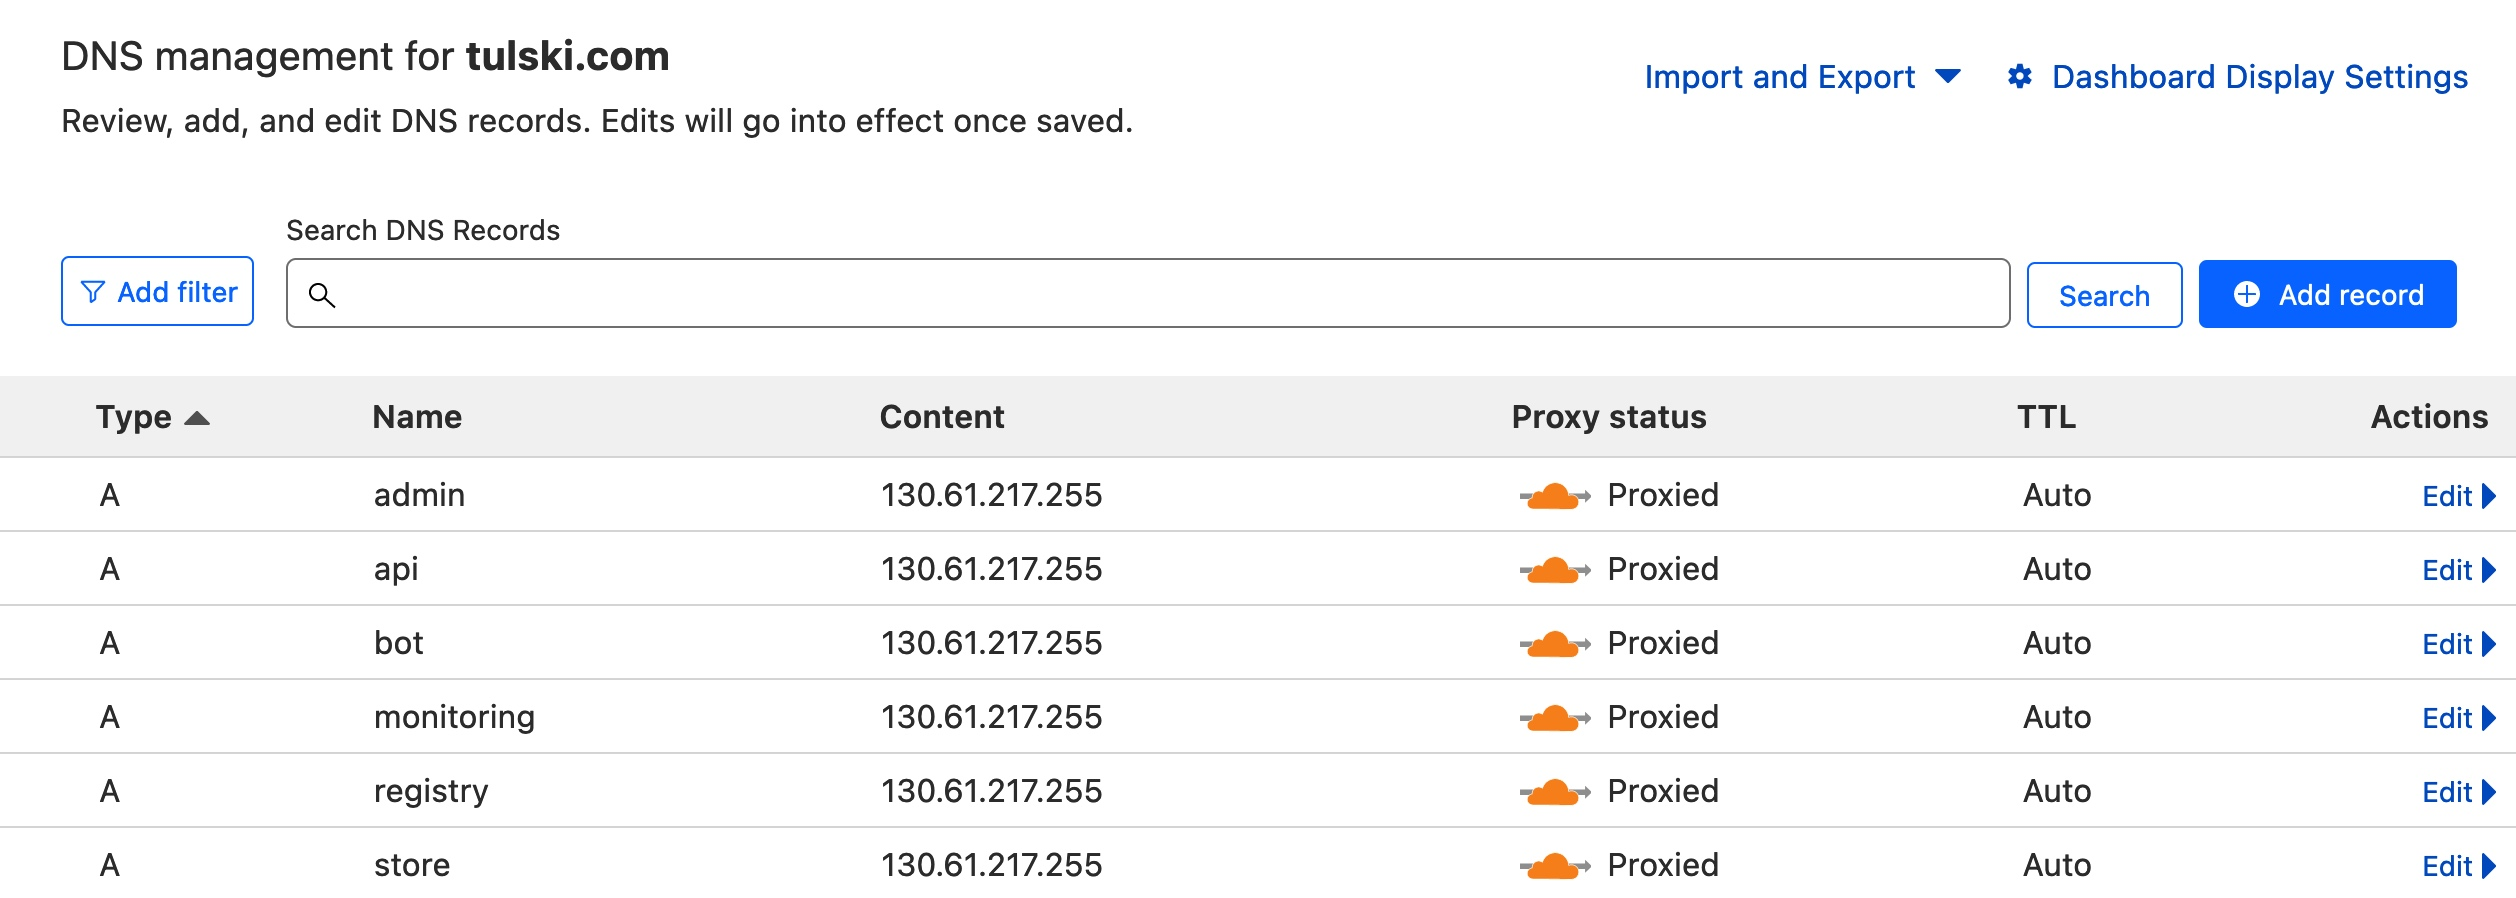
\includegraphics[width=\textwidth]{img/dns-tulski-com}
    \caption{Tabela rekordów DNS dla domeny tulski.com}
    \label{fig:dns-tulski-com}
\end{figure}

\subsection{Monitoring}\label{subsec:monitoring}

\todo{Observability Plane}

\begin{listing}[H]
    \begin{minted}[xleftmargin=10pt,linenos]{bash}
helm install observability \
    -f observability/values.yaml \
    --set "grafana.adminPassword=<adminPassword>" \
    -n observability \
    --create-namespace \
    prometheus-community/kube-prometheus-stack
    \end{minted}
    \caption{Polecenie instalujące pakiet prometheus-community/kube-prometheus-stack}
    \label{lst:helm-install-observability}
\end{listing}

%\begin{figure}[p]
%    \begin{figure}[H]
%        \centering
%        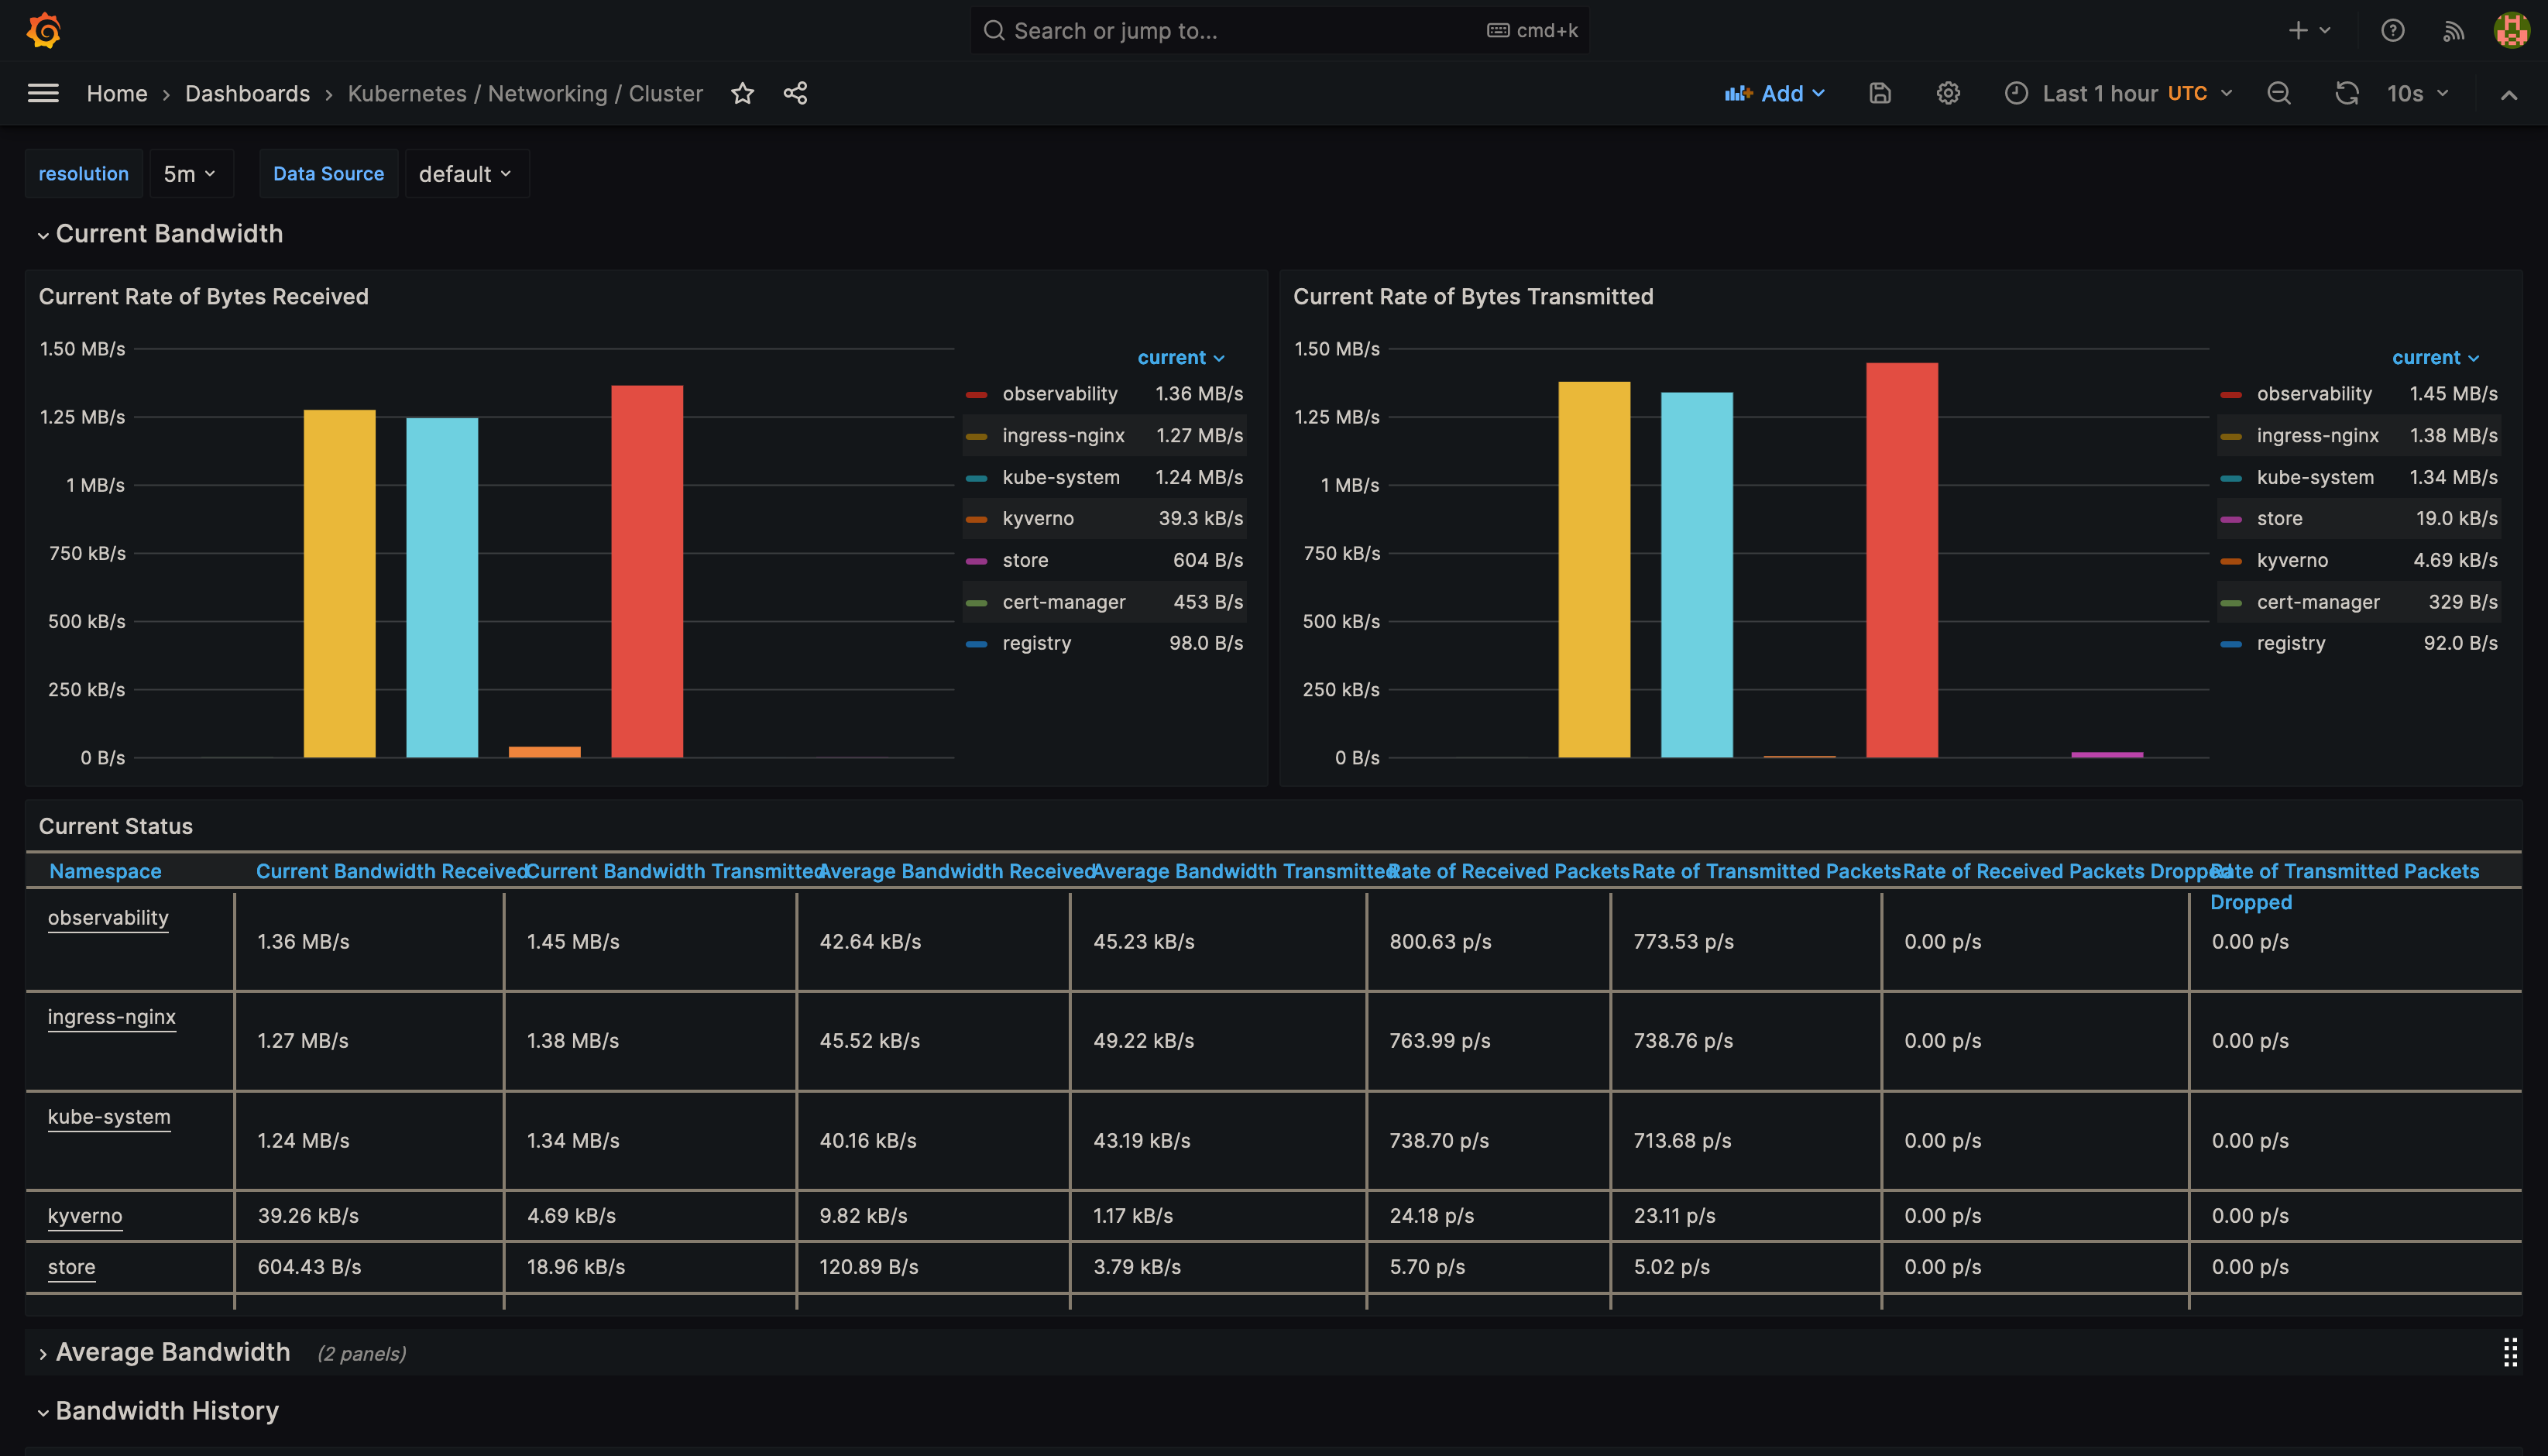
\includegraphics[width=\textwidth]{img/grafana-kubernetes-networking-cluster-dashboard}
%        \caption{Dashboard Kubernetes / Networking / Cluster}
%        \label{fig:grafana-kubernetes-networking-cluster-dashboard}
%    \end{figure}
%
%    \begin{figure}[H]
%        \centering
%        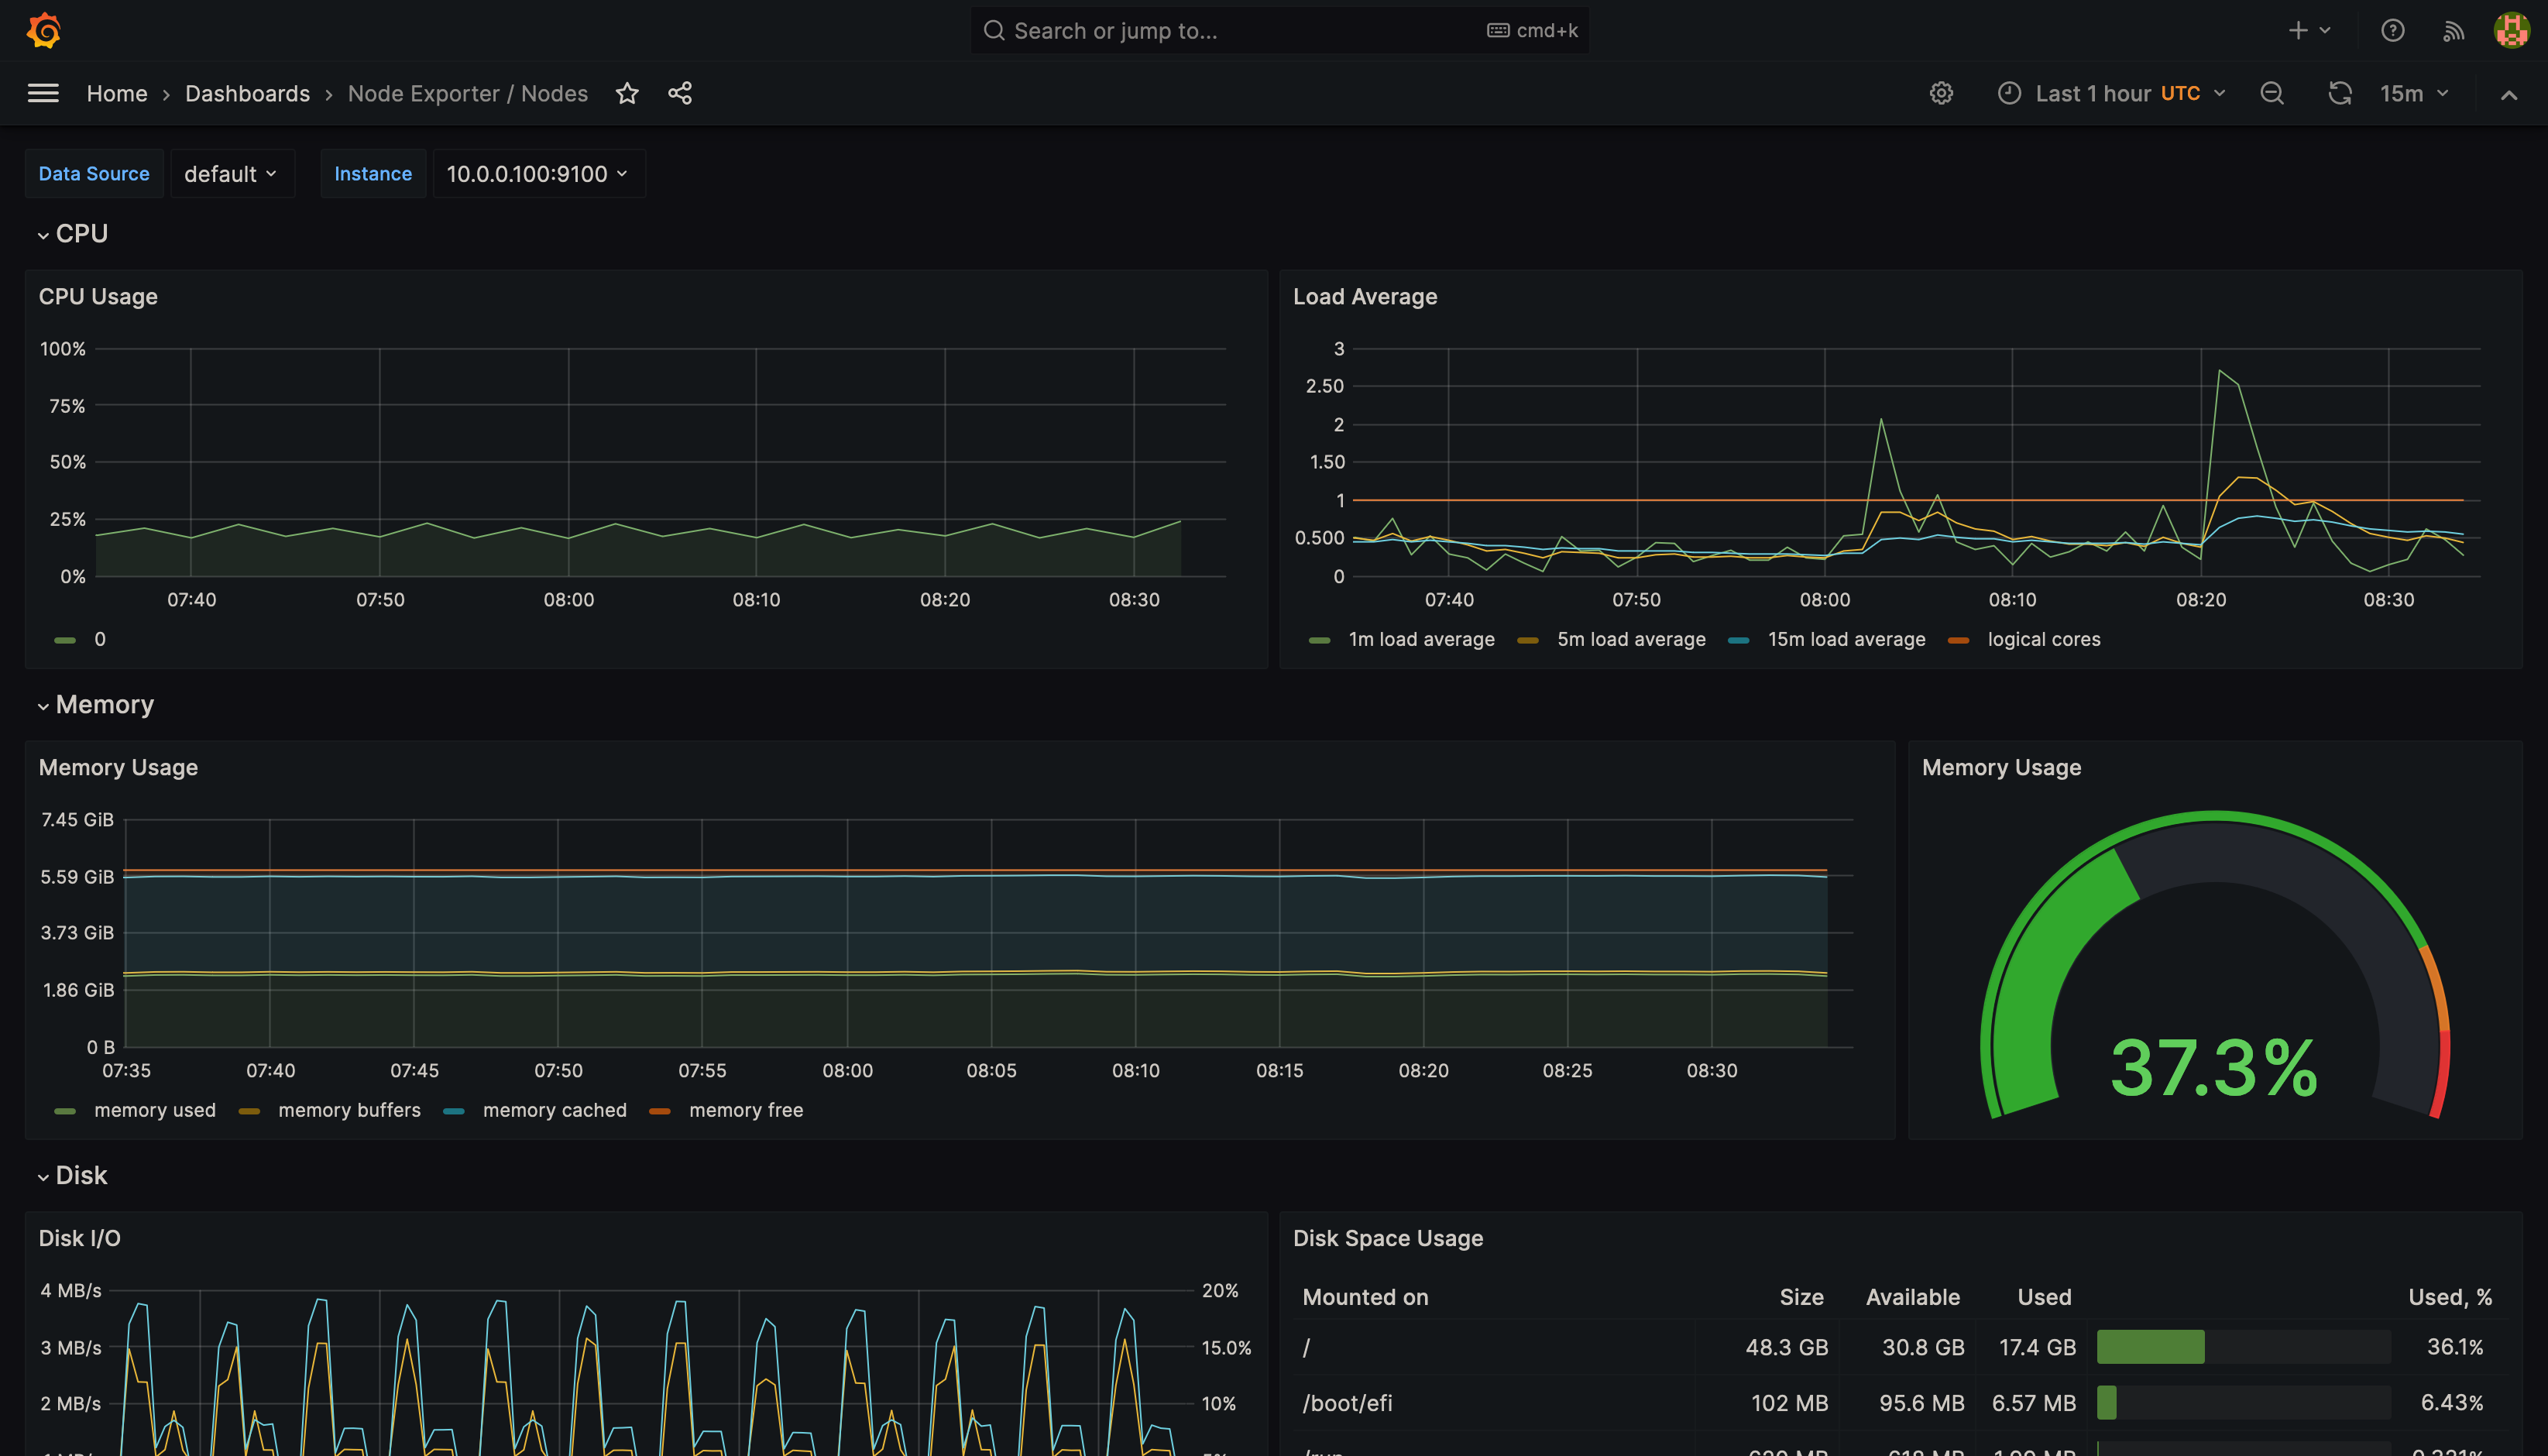
\includegraphics[width=\textwidth]{img/grafana-node-explorer-dashboard}
%        \caption{Dashboard Node Exporter / Nodes}
%        \label{fig:grafana-node-exlorer-dashboard}
%    \end{figure}
%\end{figure}

\subsection{Cert-Manager}\label{subsec:cert-manager-impl}

Wdrożenie cert-manager zostało zrealizowane przy użyciu narzędzia Helm.
Wykorzystano pakiet \url{jetstack/cert-manager} w wersji 1.13.1 (zob. listing~\ref{lst:helm-install-cert-manager}).

\begin{listing}[H]
    \begin{minted}[xleftmargin=10pt,linenos]{bash}
helm install cert-manager \
    --version v1.13.1 \
    --set installCRDs=true \
    --namespace cert-manager \
    --create-namespace \
    jetstack/cert-manager
    \end{minted}
    \caption{Polecenie instalujące pakiet jetstack/cert-manager}
    \label{lst:helm-install-cert-manager}
\end{listing}

\subsection{Docker Registry}\label{subsec:docker-registry}

\todo{Docker Registry}

\subsection{Store}\label{subsec:store}

\subsubsection{Przestrzeń nazw}

Przestrzenią nazw (ang. \emph{namespace}) nazywamy zbiór znaków (nazw) należących do jednego kontekstu.
Ich stosowanie umożliwia lepszą organizację i izolację zasobów, co przyczynia się do podniesienia bezpieczeństwa.
W środowisku Kubernetes przestrzenie nazw umożliwiają segmentację jednego klastra na mniejsze, logicznie wyizolowane jednostki.
Przestrzenie nazw mogą reprezentować środowiska różnych klientów (\emph{tenants}) lub środowiska na różnych poziomach (np. testowe i produkcyjne).

Opisywana platforma posiada przestrzeń nazw o nazwie \url{store}, która zawiera wszystkie elementy niezbędne do działania sklepu internetowego \url{store.tulski.com}.
Przestrzeń \url{store} została stworzona poprzez zaaplikowanie manifestu (zob. listing~\ref{lst:store-namespace}).

\begin{listing}[H]
    \inputminted[xleftmargin=20pt,linenos]{yaml}{code/store-namespace.yaml}
    \caption{Manifest tworzący przestrzeń nazw store}
    \label{lst:store-namespace}
\end{listing}

\subsubsection{Baza danych}\label{subsubsec:baza-danych}

Dane sklepu internetowego są fizycznie przechowywane na dyskach maszyn wirtualnych.
W CLI MicroK8s aktywowano dodatek Hostpath-Storage (zob. listing~\ref{lst:enable-hostpath-storage}), który udostępnia katalog hosta woluminom Kubernetes tj. PersistentVolumes.

\begin{listing}[H]
    \begin{minted}[xleftmargin=10pt,linenos]{bash}
microk8s enable hostpath-storage
    \end{minted}
    \caption{Polecenie aktywujące dodatek Hostpath-Storage}
    \label{lst:enable-hostpath-storage}
\end{listing}

\noindent Bazą danych jest PostgreSQL zainstalowany przy użyciu menadżera pakietów Helm.
Poleceniem \autoref{lst:helm-install-store-db} zainstalowano pakiet \url{bitnamicharts/postgresql} w przestrzeni \url{store}.

\begin{listing}[H]
    \begin{minted}[xleftmargin=10pt,linenos]{bash}
helm install store-db \
    --set auth.postgresPassword="<postgres-password>" \
    --set auth.username="store-db-admin" \
    --set auth.password="<password>" \
    --set auth.database="store" \
    --set metrics.enabled=true \
    --set metrics.serviceMonitor.enabled=true \
    --set metrics.serviceMonitor.namespace="observability" \
    --set metrics.serviceMonitor.labels.release="observability" \
    -n store \
    oci://registry-1.docker.io/bitnamicharts/postgresql
    \end{minted}
    \caption{Polecenie instalujące pakiet bitnamicharts/postgresql}
    \label{lst:helm-install-store-db}
\end{listing}

\subsubsection{Backend}

Backend, w rozumieniu architektury wielowarstwowej, pełni kluczowy element systemu informatycznego.
To warstwa stanowiąca zaplecze technologiczne, która w oparciu na zdefiniowanych regułach biznesowych, odpowiada za obsługę żądań klientów oraz przetwarza dane w sposób zapewniający ich spójność.

Serwer dostarczany przez projekt Medusa nie wymagał żadnych modyfikacji.
Jedynym wymogiem do jego uruchomienia było wybranie i dołączenie odpowiednich wtyczek (ang. \emph{plugins}) odpowiedzialnych za zarządzanie zamówieniami oraz obsługę płatności.
W tym celu zastosowano odpowiednio medusa-fulfillment-manual  i medusa-payment-manual (zob. \autoref{lst:medusa-config-fulfillment-payment}).
Obie te wtyczki można postrzegać jako atrapy (ang. \emph{mocks}), które umożliwiają funkcjonowanie serwera bez konieczności integracji z rzeczywistymi serwisami, takimi jak Stripe czy PayPal.

\begin{listing}[H]
    \begin{minted}[xleftmargin=20pt,linenos]{js}
const plugins = [
    `medusa-fulfillment-manual`,
    `medusa-payment-manual`,
    // ...
];
    \end{minted}
    \caption{Konfiguracja pluginów medusa-fulfillment-manual i medusa-payment-manual}
    \label{lst:medusa-config-fulfillment-payment}
\end{listing}

Aby backend mógł zostać uruchomiony w środowisku Kubernetes, koniecznie było jego skonteneryzowania.
Proces ten został zrealizowany przy użyciu narzędzia Docker.
W tym celu stworzono plik Dockerfile (zob. listing~\ref{lst:code-dockerfile-backend}), który definiuje wszystkie kroki budowania obrazu kontenera.
Plik Dockerfile rozpoczyna się od określenia obrazu bazowego, czyli \url{node:18-alpine}.
Następnie, w kolejnych etapach \url{deps}, \url{builder} i \url{runner}, są kolejno instalowane zależności NPM, budowany jest kod aplikacji oraz przygotowywane jest środowisko uruchomieniowe serwera.

\begin{listing}[H]
    \inputminted[xleftmargin=20pt,linenos]{docker}{code/Dockerfile.backend}
    \caption{Plik Dockerfile.backend}
    \label{lst:code-dockerfile-backend}
\end{listing}

Backend został zainstalowany i skonfigurowany w środowisku Kubernetes.
Wszystkie komponenty i mechanizmy, które składają się na to wdrożenie, zostały przedstawione na rysunku~\ref{fig:kubernetes-backend}.
Wdrożenie odbywa się przez Deployment, co umożliwia automatyzację i skalowanie aplikacji.
Komunikacja z serwisem odbywa się poprzez NGINX Virtual Server, który szyfruje dane za pomocą certyfikatu TLS wygenerowanego przez Cert-Manager.
Backend korzysta z bazy danych PostgresSQL (zob. \autoref{subsubsec:baza-danych}).
Obserwowalność działania aplikacji zapewnia Prometheus Service Monitor.
Sekrety aplikacji są bezpiecznie zarządzane za pomocą mechanizmów Kubernetes Secrets.

\begin{figure}[H]
    \centering
    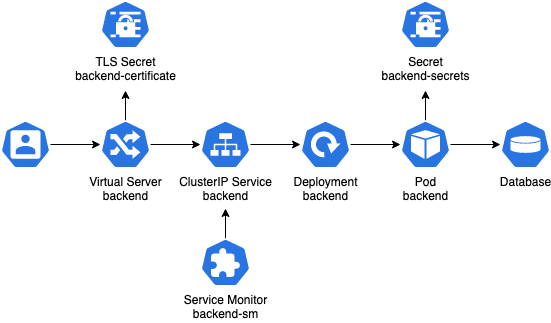
\includegraphics[width=\textwidth]{img/kubernetes-backend}
    \caption{Backend w środowisku Kubernetes}
    \label{fig:kubernetes-backend}
\end{figure}

\subsubsection{Panel administratora}

Panel administratora to kolejny element rozbudowanego ekosystemu Medusa, który jest dostarczany w formie wtyczki (ang. \emph{plugin}).
Panel stanowi graficzny interfejs dla Admin REST API. Jego zastosowanie umożliwia łatwe zarządzanie produktami, zamówieniami oraz ustawieniami sklepu.

Wtyczka panelu administratora, skonfigurowana w plikach serwera backend (zob. listing~\ref{lst:medusajs-admin-plugin}), może być uruchomiona równolegle z backendem, lub jako niezależny serwer.
Zdecydowano się na drugą opcję, ponieważ pozwala ona na niezależne skalowanie obu aplikacji.

\begin{listing}[H]
        \begin{minted}[xleftmargin=20pt,linenos]{js}
const plugins = [
    {
        resolve: "@medusajs/admin",
        options: { /* ... */ },
    },
    // ...
];
        \end{minted}
    \caption{Dołączenie wtyczki @medusajs/admin}
    \label{lst:medusajs-admin-plugin}
\end{listing}

Panel administratora jest budowany do postaci statycznych plików HTML, CSS i JavaScript, które następnie są hostowane przez serwer NGINX (zob. listing~\ref{lst:medusajs-admin-dockerfile}).

\begin{listing}[H]
    \inputminted[xleftmargin=20pt,linenos]{docker}{code/Dockerfile.admin}
    \caption{Plik Dockerfile panelu administratora}
    \label{lst:medusajs-admin-dockerfile}
\end{listing}

Panel administratora w środowisku Kubernetes funkcjonuje jako osobna jednostka wdrożeniowa, niezależna od backendu.
Wykorzystuje NGINX Virtual Server z szyfrowaniem TLS. Certyfikat jest generowany przez Cert-Manager.
Architektura obejmuje service oraz deployment z jednym podem, co przedstawiano na rysunku~\ref{fig:kubernetes-admin}.

\begin{figure}[H]
    \centering
    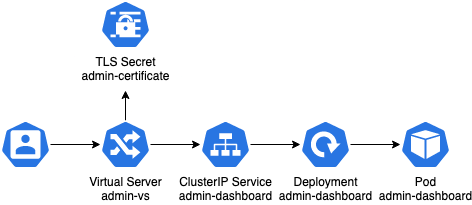
\includegraphics[width=0.9\textwidth]{img/kubernetes-admin-panel}
    \caption{Panel administratora w środowisku Kubernetes}
    \label{fig:kubernetes-admin}
\end{figure}

\subsubsection{Witryna internetowa}

Witryna internetowa, będąca warstwą prezentacyjną systemu, odgrywa kluczową rolę w interakcji z klientem końcowym.
Główny zadaniem tej witryny jest prezentacja oferowanych produktów oraz umożliwienie użytkownikom przeprowadzenia procesu zakupowego.
Projekt Medusa dostarcza szablon witryny sklepu internetowego w formie osobnego projektu o nazwie Storefront.
Storefront, jako graficzny interfejs dla Store REST API, stanowi integralną część reszty systemu Medusa.

Witryna internetowa, analogicznie do części serwerowej oraz panelu administratora, została zintegrowana w strukturze całej platformy poprzez proces skonteneryzowania i wdrożenia w środowisku Kubernetes (zob. rysunek~\ref{fig:kubernetes-storefront}).

\begin{figure}[H]
    \centering
    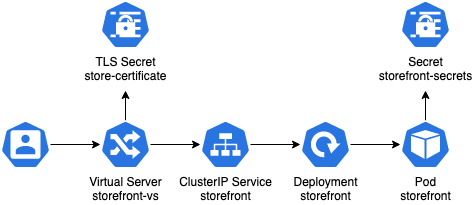
\includegraphics[width=\textwidth]{img/kubernetes-storefront}
    \caption{Witryna internetowa w środowisku Kubernetes}
    \label{fig:kubernetes-storefront}
\end{figure}

Rysunek~\ref{fig:storefront-homepage} przedstawia stronę domową sklepu, akcentując powód jego powstania, czyli niniejszą pracę dyplomową.
Natomiast rysunek~\ref{fig:storefront-products} ilustruje stronę z produktami, ukazując sposób prezentacji asortymentu.
Obie strony razem podkreślają znaczenie estetyki i funkcjonalności w interfejsie użytkownika sklepu internetowego.

\begin{figure}[p]
    \begin{figure}[H]
        \centering
        \fbox{\includegraphics[width=\textwidth]{img/storefront-homepage}}
        \caption{Strona domowa sklepu internetowego}
        \label{fig:storefront-homepage}
    \end{figure}

    \begin{figure}[H]
        \centering
        \fbox{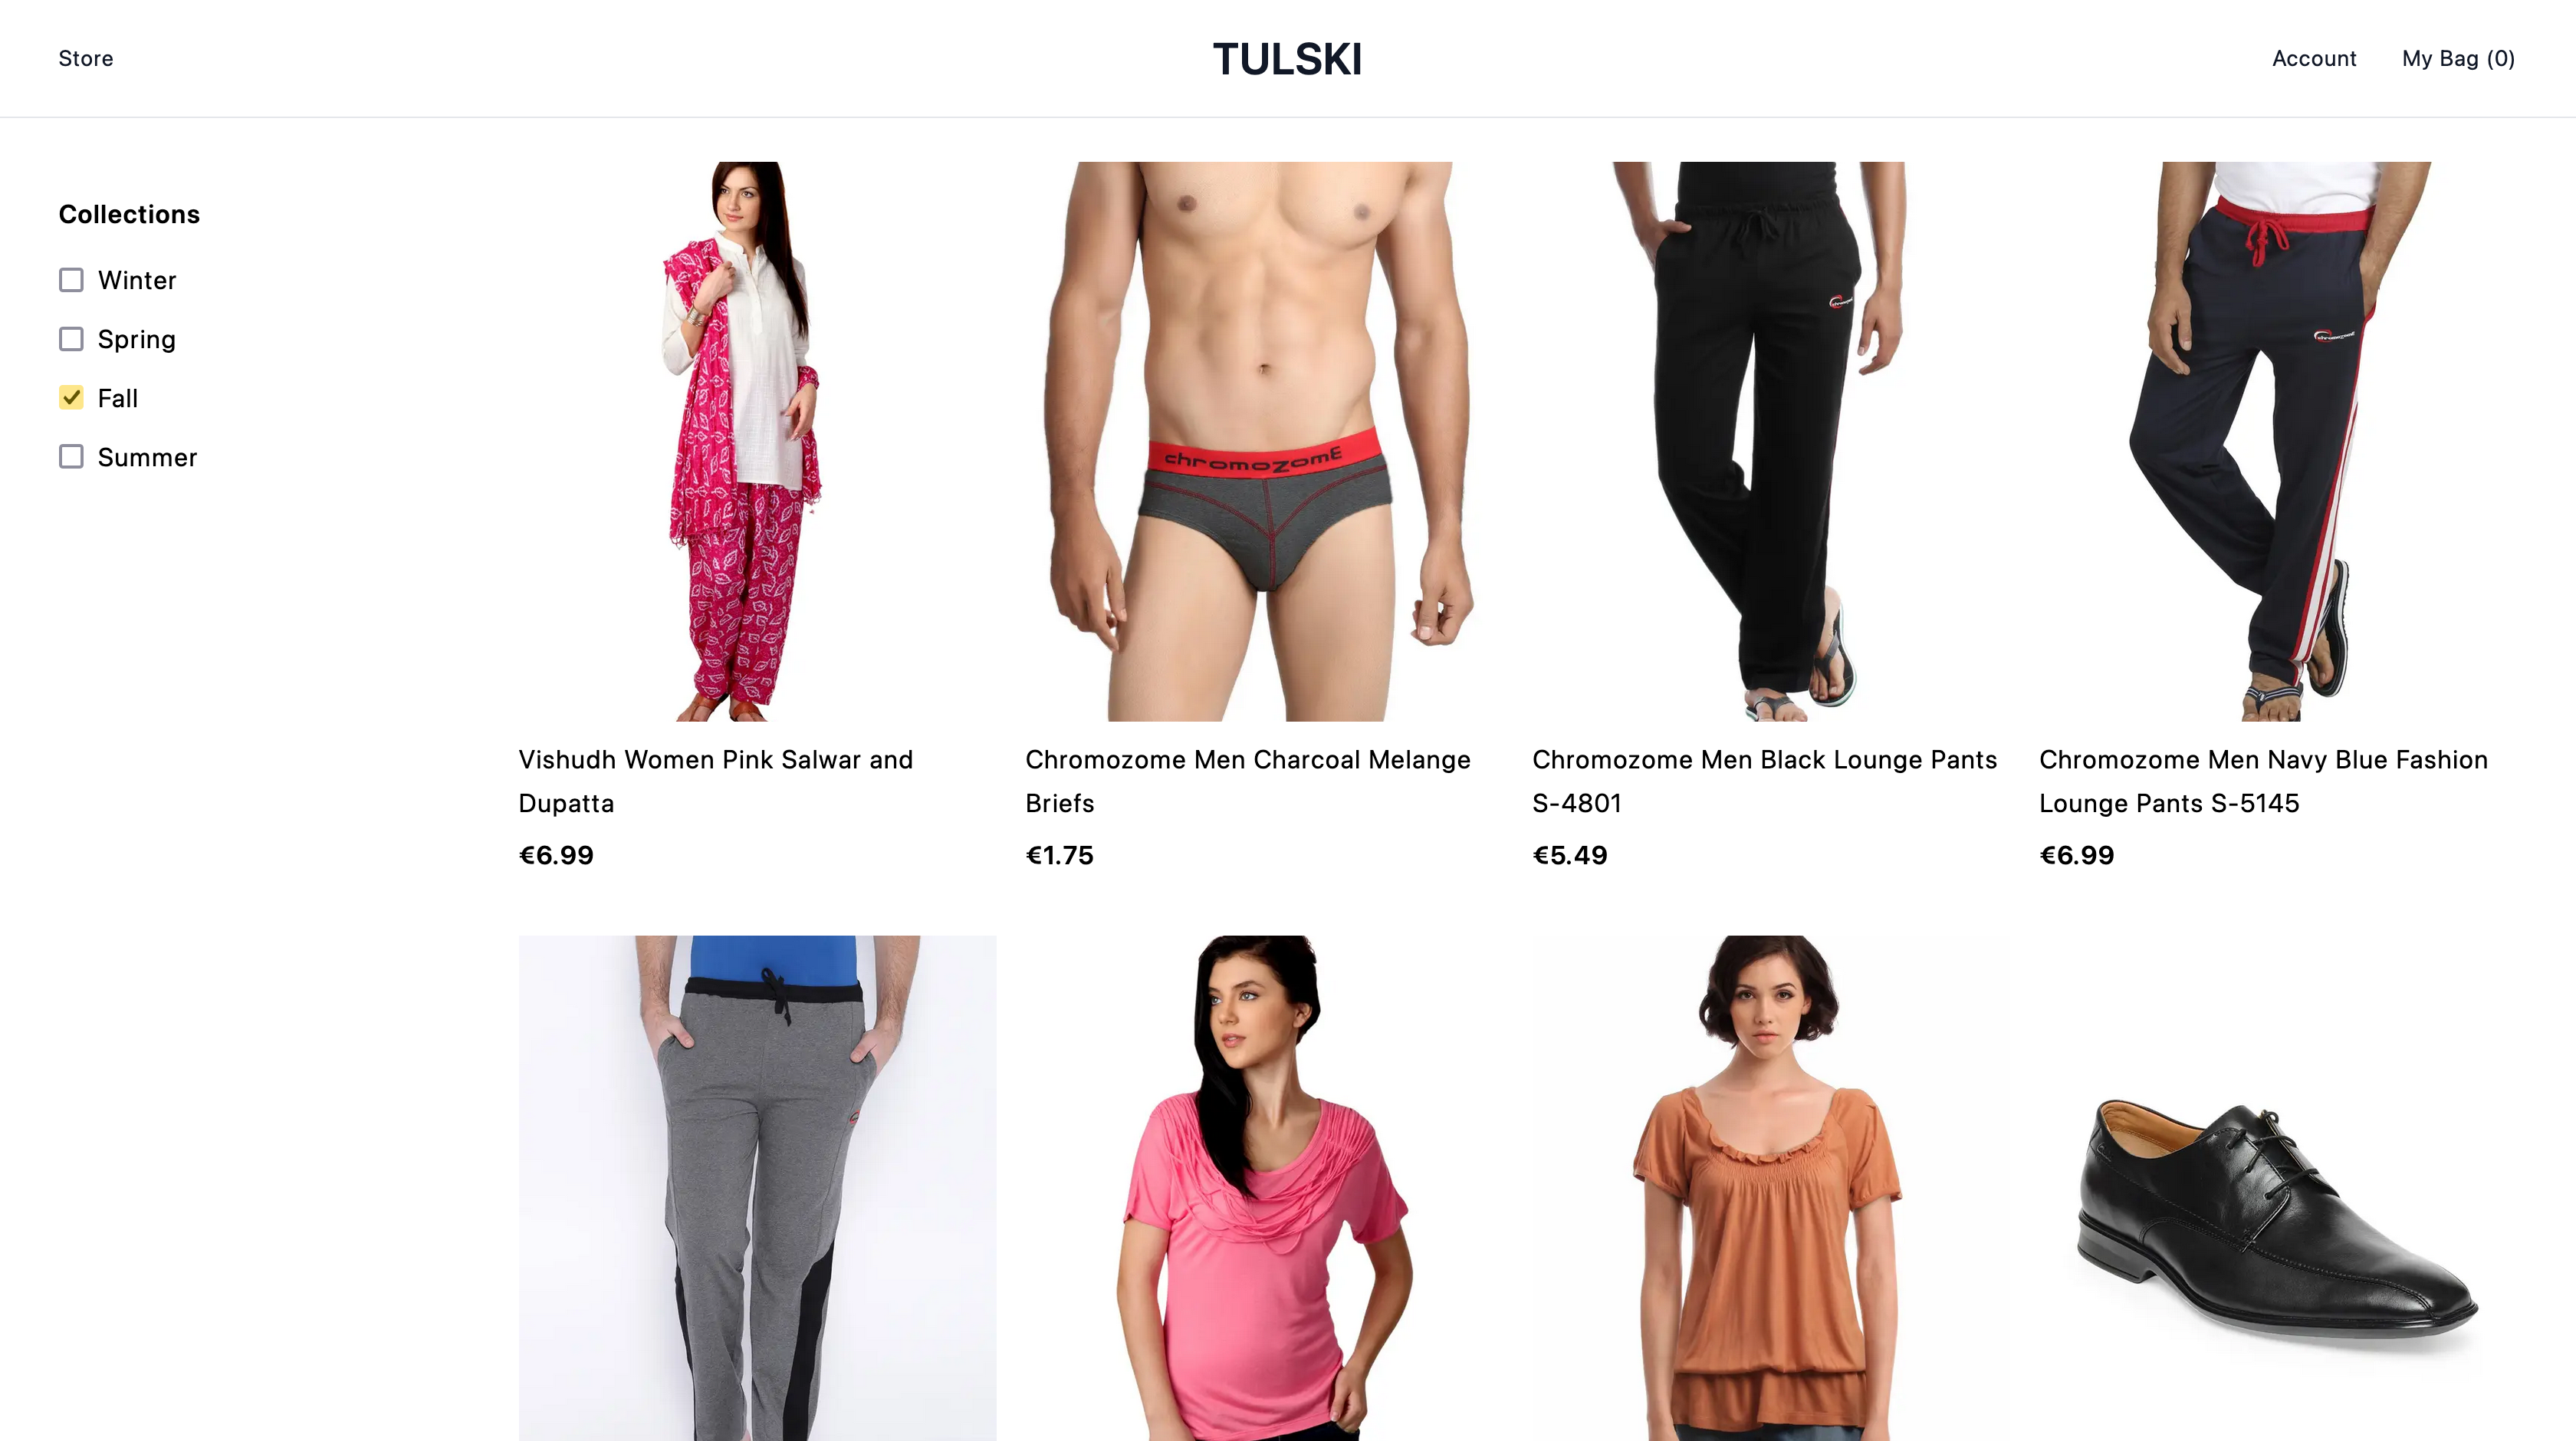
\includegraphics[width=\textwidth]{img/storefront-products}}
        \caption{Strona z produktami sklepu internetowego}
        \label{fig:storefront-products}
    \end{figure}
\end{figure}

\subsubsection{Import produktów}

Sklep internetowy uzupełniono 11440 przykładowymi produktami (zob. listing~\ref{lst:store-count-products}), które pozyskano z zbioru danych~\citetitle*{fashion-dataset}\cite{fashion-dataset} udostępnionego przez~\citeauthor*{fashion-dataset} na platformie Kaggle.

\begin{listing}[H]
    \begin{minted}[xleftmargin=10pt,linenos]{sql}
store=> select count(*) from product;
 count
-------
 11440
(1 row)
    \end{minted}
    \caption{Zapytanie zwracające liczbę wszystkich produktów}
    \label{lst:store-count-products}
\end{listing}

\newpage


\section{Projekt i wykonanie scrapera}\label{sec:projekt-scrapera}

Niniejszy rozdział poświęcono projektowi i wykonaniu scrapera - narzędzia służącego do automatycznego zbierania danych z sklepu internetowego tulski, omówionego w \autoref{sec:projekt-platformy}.
Założono, że celem scrapera jest zgromadzenie informacji o wszystkich produktach dostępnych w sklepie internetowym, które mogą zostać wykorzystane do analizy asortymentu i cen produktów.
Kolejnym, istotnym założeniem rozdziału jest podejście typu czarnej skrzynki (ang. \emph{black-box})\cite{sekurak-testy-penetracyjne}.
Brak początkowej wiedzy na temat struktury i mechanizmów scrapowanego serwisu, jakim jest sklep internetowy tulski, nadaje realizm opisanym działaniom, odzwierciedlając warunki, w jakich najczęściej pracują osoby specjalizujące się w web scrapingu.
Poniższa część pracy jest zatem nie tylko technicznym studium przypadku, ale również wglądem w procesy myślowe i metody, które są wykorzystywane w realnych warunkach.

\subsection{Rekonesans}\label{subsec:rekonesans}

Rekonesans rozpoczął proces tworzenia scrapera, skupiając się na zrozumieniu celu, jakim jest sklep internetowy tulski.
Głównym zadaniem rekonesansu było zidentyfikowanie metod dających efektywny dostęp do interesujących danych.
Skupiono się na zrozumieniu mechanizmu ładowania i renderowania treści, strukturze zasobów oraz wykryciu potencjalnych wyzwań, które mogłyby wpłynąć na proces scrapowania.
Rekonesans jest kluczowym etapem w tworzeniu scrapera, ponieważ od niego zależą efektywność, awaryjność i stabilność narzędzia.
Przykładowo, jeśli podczas rekonesansu uda się znaleźć żądania API, które zwracają dane w formacie JSON, narzędzie będzie potencjalnie szybsze i bardziej odporne na zmiany.
Wynika to z faktu, że kontakt API zmienia się z reguły rzadziej niż interfejs graniczny użytkownika.

Kluczowym elementem rekonesansu była analiza ruchu sieciowego za pomocą narzędzi programistycznych wbudowanych w przeglądarkę internetową Firefox.
Po pierwsze, ustalono, że strona korzysta korzysta z proxy Cloudflare, co wskazuje nagłówek \emph{server} (zob. \autoref{lst:rekonesans-get-homepage}).
Po drugie, odkryto, że strona została zbudowana z wykorzystaniem frameworka Next, co wskazuje nagłówek \emph{x-powered-by} (zob. \autoref{lst:rekonesans-get-homepage}).
Wykorzystanie Next oznacza wykorzystanie React, co może sugerować dynamiczne renderowanie treści.

\begin{listing}[H]
    \begin{minted}[xleftmargin=10pt,linenos,breaklines]{bash}
$ curl -I https://store.tulski.com
HTTP/2 200
date: Sun, 17 Dec 2023 17:09:05 GMT
content-type: text/html; charset=utf-8
cache-control: private, no-cache, no-store, max-age=0, must-revalidate
vary: RSC, Next-Router-State-Tree, Next-Router-Prefetch, Next-Url, Accept-Encoding
x-powered-by: Next.js
cf-cache-status: DYNAMIC
report-to: {"endpoints":[{"url":"https:\/\/a.nel.cloudflare.com\/report\/v3 ?s=l8mwfqVrt2h%2BXJYVshGNiHz%2FIRwSCEqIgVqxZ8kBhWWqkIGQaAuYiOy9 sv4JmNEGP1%2B53j1pVTVnm%2BpX2sID4%2BRDooubYk4tibHwMUz8sjuDxll1N rjXEffI6gReu1VJV7JI"}], "group":"cf-nel", "max_age":604800}
nel: {"success_fraction":0,"report_to":"cf-nel","max_age":604800}
server: cloudflare
cf-ray: 8370c5927feb666e-AMS
alt-svc: h3=":443"; ma=86400
    \end{minted}
    \caption{Nagłówki odpowiedzi dla strony domowej sklepu tulski}
    \label{lst:rekonesans-get-homepage}
\end{listing}

Po trzecie, w trakcie rekonesansu zauważono żądania do serwera API \emph{api.tulski.com}.
Odkrycie potwierdza hipotezę o dynamicznym renderowaniu treści na stronie.
Serwer API, podobnie jak witryna internetowa, korzysta z proxy Cloudflare.
Zidentyfikowano dwa żądania, które zwracają dane o produktach w formacie JSON\@.
Jednym z zidentyfikowanych żądań jest to, które zwraca listę produktów (zob. \autoref{fig:store-get-products-list}), wykorzystując paginację.
W żądaniu rozmiar strony jest określany parametrem \emph{limit}, a pozycję startową strony - parametrem \emph{offset}.

Przeprowadzono testy metodą prób i błędów, aby określić maksymalną liczbę produktów, jaką może zwrócić API w jednej odpowiedzi.
Ustalono, że parametr \emph{limit} nie posiada ścisłej walidacji, co umożliwia pobranie znacznie większej ilości danych niż to, co zwykle pobiera klient aplikacji internetowej.
Jednakże, zauważono, że ograniczeniem podczas pobierania dużej liczby rekordów jest czas otwarcia połączenia.
W przypadkach, gdy próbowano pobrać bardzo dużą liczbę rekordów, na przykład 8500 (zob.~\autoref{lst:store-get-products-list-8500}), serwer odpowiedział statusem \emph{504 Gateway Timeout}, wskazując na przekroczenie maksymalnego dopuszczalnego czasu przetwarzania żadania.
Maksymalną liczbą rekordów jaką udało się pobrać bez błędów było 8000 (zob.~\autoref{lst:store-get-products-list-8000}).

\begin{figure}[p]
    \centering
    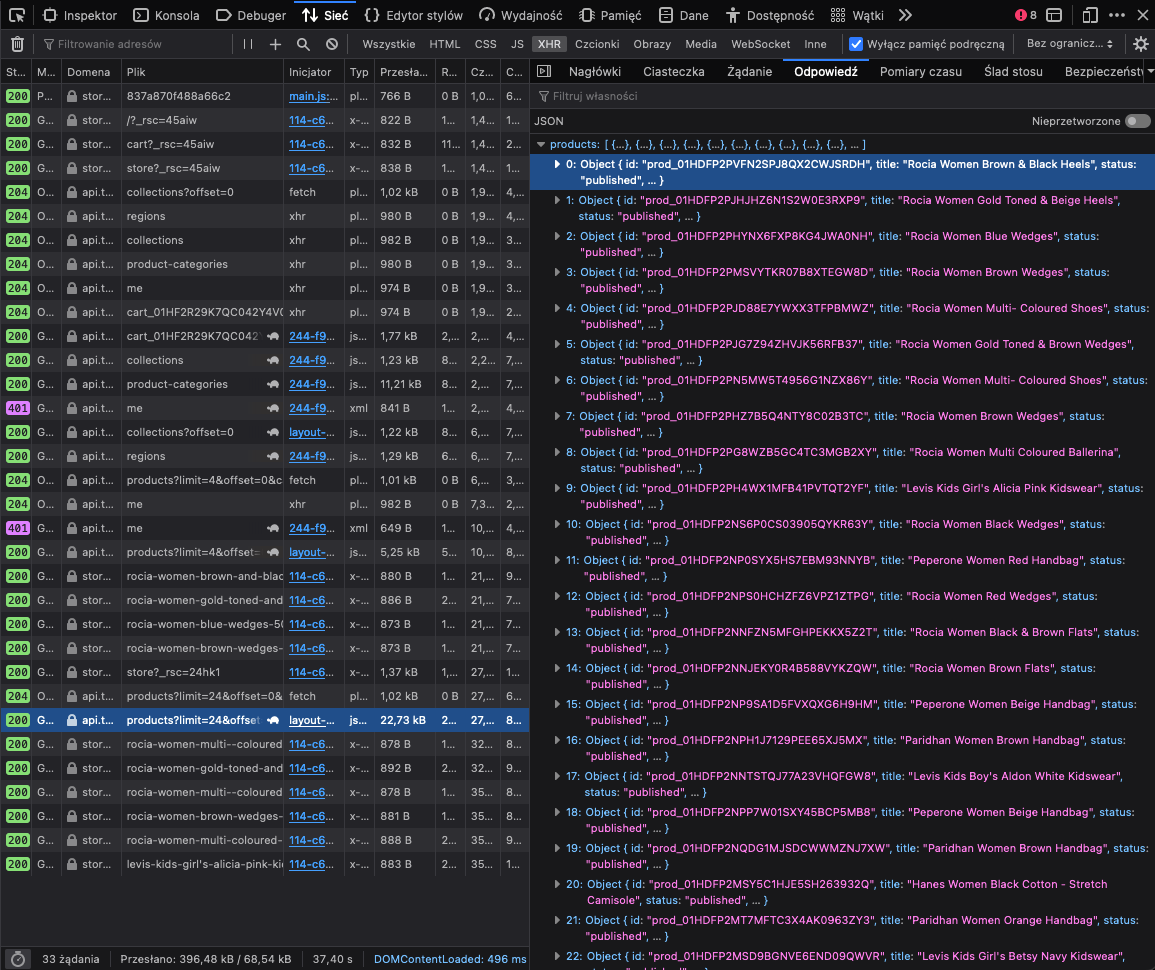
\includegraphics[width=0.8\textwidth]{img/store-get-products-list}
    \caption{Żądanie zwracające listę produktów}
    \label{fig:store-get-products-list}
\end{figure}
\begin{listing}[p]
    \begin{minted}[xleftmargin=10pt,linenos]{bash}
$ curl -X GET 'https://api.tulski.com/store/products?limit=8500' \
        -s \
        -o /dev/null \
        -w 'HTTP Code: %{http_code}\nTime Total: %{time_total}s\n'
HTTP Code: 504
Time Total: 61.691521s
    \end{minted}
    \caption{Żądanie 8500 produktów}
    \label{lst:store-get-products-list-8500}
\end{listing}
\begin{listing}[p]
    \begin{minted}[xleftmargin=10pt,linenos]{bash}
$ curl -X GET 'https://api.tulski.com/store/products?limit=8000' \
        -s \
        -o /dev/null \
        -w 'HTTP Code: %{http_code}\nTime Total: %{time_total}s\n'
HTTP Code: 200
Time Total: 60.223100s
    \end{minted}
    \caption{Żądanie 8000 produktów}
    \label{lst:store-get-products-list-8000}
\end{listing}

\newpage

Następne żądanie API, które zwróciło uwagę podczas rekonesansu, dotyczyło pobierania szczegółowych danych o produkcie (zob. \autoref{fig:store-get-product-details}).
Odpowiedź serwera na to żądanie zawiera bogaty zestaw danych o produkcie, w tym nazwę, opis, zdjęcia, linki do obrazów, metadane oraz szczegóły dotyczące rozmiarów i wariantów z ich dostępności.
Struktura danych w formacie JSON, wykorzystana w odpowiedzi (zob. Listing ~\autoref{lst:store-get-product-details-request}), jest przejrzysta i dobrze zorganizowana.
Zwracane dane wyczerpują wymagania postawione przed scraperem.

\begin{figure}[H]
    \centering
    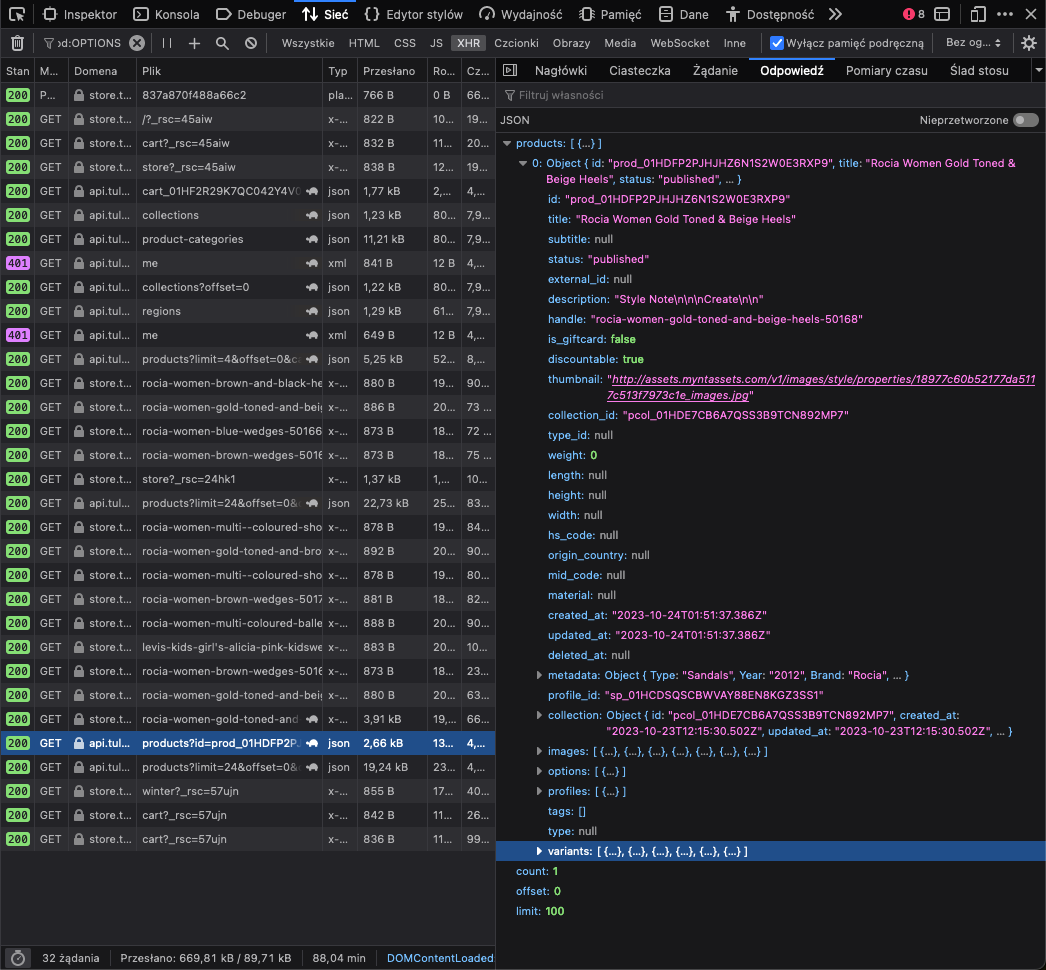
\includegraphics[width=0.8\textwidth]{img/store-get-product-details}
    \caption{Żądanie po szczegóły produktu}
    \label{fig:store-get-product-details}
\end{figure}
\begin{listing}[H]
    \begin{minted}[xleftmargin=10pt,linenos,breaklines]{bash}
$ curl -G -d "id=prod_01HDFP2PJHJHZ6N1S2W0E3RXP9" \
        "https://api.tulski.com/store/products"
{"products": [{"id": "prod_01HDFP2PJHJHZ6N1S2W0E3RXP9", "title": "Rocia Women Gold Toned & Beige Heels", "subtitle": null, "status": "published", "external_id": null, "description": "Style Note\n\n\nCreate\n\n", "handle": "rocia-women-gold-toned-and-beige-heels-50168", "is_giftcard": false, "discountable": true, "thumbnail": ...
    \end{minted}
    \caption{Struktura JSON odpowiedzi na żądanie po szczegóły produktu}
    \label{lst:store-get-product-details-request}
\end{listing}

\subsection{Implementacja}\label{subsec:scraper-implementation}

Po uzyskaniu odpowiedniej ilości informacji rozpoczęto proces tworzenia scrapera.
Podczas rekonesansu ustalono, że strona jest renderowana dynamicznie i pobierane dane z końcówek API, które zwracają dane w formacie JSON, dlatego zdecydowano się na scraping API\@.
Wykorzystano język programowania TypeScript, środowisko uruchomieniowe Node.js i bibliotekę got.

\subsubsection{Konfiguracja klienta HTTP}

Skonfigurowano klienta HTTP \texttt{storeClient}, który wysyła żądania do serwera API z nagłówki typowymi dla przeglądarki internetowej.
Działanie to miało na celu jak najwierniejsze odwzorowanie śladu i zachowań scrapera na wzór klienta przeglądarkowego, co zwiększa jego dyskrecję podczas działania.
Ponadto dodano logowanie żądań i odpowiedzi, co znacząco ułatwia proces debugowania, monitorowania i identyfikacji potencjalnych błędów.
Konfiguracja została przedstawiona na \autoref{lst:store-http-client-config}.

\begin{listing}[H]
    \begin{minted}[xleftmargin=10pt,linenos,breaklines]{typescript}
const storeClient: typeof got = got.extend({
  prefixUrl: "https://api.tulski.com/",
  hooks: {
    beforeRequest: [requestLogger(logger)],
    afterResponse: [responseLogger(logger)],
  },
  headers: {
    "User-Agent":
      "Mozilla/5.0 (Macintosh; Intel Mac OS X 10.15; rv:121.0) Gecko/20100101 Firefox/121.0",
    Accept: "*/*",
    "Accept-Language": "en-US,en;q=0.7,pl;q=0.3",
    "Accept-Encoding": "gzip, deflate, br",
    "Access-Control-Request-Method": "GET",
    DNT: "1",
    "Sec-GPC": "1",
    Connection: "keep-alive",
    "Sec-Fetch-Dest": "empty",
    "Sec-Fetch-Mode": "cors",
    "Sec-Fetch-Site": "same-site",
    Pragma: "no-cache",
    "Cache-Control": "no-cache",
  },
});
    \end{minted}
    \caption{Konfiguracja klienta HTTP storeClient}
    \label{lst:store-http-client-config}
\end{listing}

\subsubsection{Funkcja pobierająca listę produktów}

Następnie, zaimplementowano funkcje \texttt{getProductsList} służącą do pobierania listy produktów (zob. \autoref{lst:store-http-client-getProductsList}).
Wykorzystano Pagination API biblioteki got\cite{got-paginate-docs}, które pozwala na iteracyjne pobieranie kolejnych pozycji z listy produktów.
Lista 500 produktów jest zwracana w żądaniu \texttt{GET /store/products}.
Funkcja \texttt{transform} parsuje otrzymaną odpowiedź (\texttt{Response}) do listy produktów.
Funkcja \texttt{paginate} zwraca atrybuty wskazujące na następną stronę. Wylicza nową wartość parametru offset wykorzystując aktualną długość listy produktów i wartość offset.

\begin{listing}[H]
    \begin{minted}[xleftmargin=10pt,linenos,breaklines]{typescript}
export const getProductsList = () => {
  return storeClient.paginate({
    url: "store/products",
    searchParams: {
      currency_code: "eur",
      is_giftcard: false,
      limit: 500
    },
    pagination: {
      transform: (response: Response<string>): ProductListing[] => {
        return JSON.parse(response.body).products;
      },
      paginate: ({ response, currentItems }) => {
        if (currentItems.length === 0) {
          return false;
        }
        const searchParams = response.request.options
          .searchParams as URLSearchParams;
        const previousOffset = Number(searchParams?.get("offset") ?? 0);
        return {
          searchParams: {
            offset: previousOffset + currentItems.length,
          },
        };
      },
      countLimit: 5000,
      // Wait before making another request to prevent rate limiting
      backoff: 500,
      requestLimit: 1000,
      stackAllItems: false,
    },
  });
};
    \end{minted}
    \caption{Funkcja pobierająca listę produktów}
    \label{lst:store-http-client-getProductsList}
\end{listing}

\subsubsection{Funkcja pobierająca szczegóły produktu}

Ostatnią zaimplementowaną funkcją wykorzystującą \texttt{storeClient} jest funkcja \texttt{get-\\ProductDetails} (zob. \autoref{lst:store-http-client-getProductDetails}).
Pobiera ona szczegółowe dane o produkcie z wskazanym w argumencie identyfikatorze.
Wykorzystuje żądanie \texttt{GET /store/products/\\{{productId}}} odkryte podczas rekonesansu.

\begin{listing}[H]
    \begin{minted}[xleftmargin=10pt,linenos,breaklines]{typescript}
export const getProductDetails = (
  productId: string,
): CancelableRequest<ProductResponse> => {
  return storeClient
    .get(`store/products/${productId}`, {
      searchParams: {
        currency_code: "eur",
      },
    })
    .json();
};
    \end{minted}
    \caption{Funkcja pobierająca szczegóły produktu}
    \label{lst:store-http-client-getProductDetails}
\end{listing}

\subsubsection{Mechanizm kolejkujący zadania}

Scraper wyposażono w mechanizm kolejkujący zadania.
Jest to powszechnie znane i używane rozwiązanie w tego rodzaju oprogramowaniu.
Należy pamiętać, że domeną scraperów jest bardzo duża ilość asynchronicznych procesów (m.in. zapytania HTTP).
Wybranymi zaletami mechanizmów kolejkujących w scraperach są:
\begin{itemize}
    \item efektywne zarządzanie zasobami (np. karty sieciowej),
    \item kontrola nad liczbą i częstotliwością zapytań do serwera docelowego, co jest istotne dla uniknięcia blokowania,
    \item ułatwiona monitoring i obsługa błędów poprzez możliwość ponownego przetwarzania zadania,
    \item skalowalność i elastyczność scrapera.
\end{itemize}
\noindent \autoref{lst:queue-implementation} przedstawia implementację klasy \texttt{Queue} reprezentującej asynchroniczną kolejkę zadań.
Wykorzystano zewnętrzną bibliotekę queue, która została dodatkowo przykryta własną warstwą abstrakcji, tak aby ułatwić jej dalsze wykorzystanie.

\begin{listing}[p]
    \begin{minted}[xleftmargin=10pt,linenos,breaklines]{typescript}
import { default as ExternalQueue } from "queue";

export interface QueueOptions {
  concurrency: number;
}

export class Queue<T> {
  private readonly queue: ExternalQueue;

  constructor(options: QueueOptions) {
    this.queue = new ExternalQueue({
      concurrency: options.concurrency,
      autostart: true,
      results: [],
    });
  }

  get results() {
    return (this.queue.results || []).filter((el) => el !== null);
  }

  get finishedJobsCount() {
    return this.results.length;
  }

  get jobsCount() {
    return this.queue.length;
  }

  set onSuccess(callback: () => void) {
    this.queue.addEventListener("success", callback);
  }

  push(job: () => Promise<T>) {
    this.queue.push(job);
  }

  async waitUntilEnd() {
    await new Promise<void>((resolve, reject) => {
      this.queue.addEventListener("end", () => {
        resolve();
      });
    });
  }
}

    \end{minted}
    \caption{Implementacja klasy Queue}
    \label{lst:queue-implementation}
\end{listing}

\subsubsection{Zapis danych}

Pobrane dane należy zapisać.
W tym celu zaimplementowano klasę \texttt{LocalDirectory-\\Bucket} (zob. \autoref{lst:storage-save-product}).
Jej metoda save zapisuje otrzymane dane w postaci tekstowej pod wskazaną ścieżką.
Pliki są zapisywane w jednym katalogu w lokalnym systemie plików.

Użycie powszechnie znanej koncepcji \texttt{Bucket} jako interfejsu pozostawia oprogramowanie otwarte na zmiany.
Scraper może wykorzystywać dowolny system plików, na przykład Amazon S3 lub Google Cloud Storage.

\begin{listing}[p]
    \begin{minted}[xleftmargin=10pt,linenos,breaklines]{typescript}
import { writeFile, mkdir, access } from "fs/promises";
import path from "node:path";

export interface LocalDirectorBucketConfig {
  directory: string;
}

export class LocalDirectoryBucket implements Bucket {
  private directoryExists: undefined | true;

  constructor(private readonly config: LocalDirectorBucketConfig) {}

  async save(filepath: string, data: string | Record<any, any>) {
    await this.ensureDirExists();
    const stringifiedData =
      typeof data === "string" ? data : JSON.stringify(data);
    const fullPath = path.join(this.config.directory, filepath);
    return writeFile(fullPath, stringifiedData);
  }

  private async ensureDirExists() {
    if (this.directoryExists) {
      return;
    }
    try {
      await access(this.config.directory);
    } catch (error: any) {
      if (error.code === "ENOENT") {
        await mkdir(this.config.directory, { recursive: true });
      }
    }
    this.directoryExists = true;
  }
}
    \end{minted}
    \caption{Klasa LocalDirectoryBucket}
    \label{lst:storage-save-product}
\end{listing}

\newpage

\subsubsection{Punkt wejścia programu}

Punktem wejścia programu jest samowywołująca się funkcja asynchroniczna (ang. \emph{Self-Invoking Function}) zarządzająca procesem scrapowania (zob. \autoref{lst:scraper-main}).
Opisywana funkcja kolejno:

\begin{enumerate}
    \item Tworzy zmienną \texttt{timestamp}, która przechowuje znacznik czasowy (ang. \emph{timestamp}) identyfikujący bieżące uruchomienie programu.
    \item Tworzy zmienną \texttt{outDir}, która będzie ścieżką katalogu wyjściowego.
    Składową \texttt{outDir} jest wcześniej stworzony identyfikator.
    \item Inicjuje \texttt{bucket} jako instancję klasy \texttt{LocalDirectoryBucket} z ścieżką \texttt{outDir}.
    \item Inicjuje \texttt{queue} jako instancję klasy \texttt{Queue} z ograniczeniem równolegle wykonywanych zadań do 100.
    \item Definuje akcję wykonywaną po każdym skończonym zadaniu w kolejce, która loguje jej aktualny stan.
    \item Dla każdego produktu z listy produktów (\texttt{getProductsList}) dodaje do kolejki zadanie, które
    pobiera szczegóły produktu (\texttt{getProductDetails}) i zapisuje je do pliku JSON\@.
\end{enumerate}

\begin{listing}[H]
    \begin{minted}[xleftmargin=10pt,linenos,breaklines]{typescript}
(async () => {
  const timestamp = new Date();
  const outDir = path.join(
    "out",
    timestamp.toISOString().replace(/\D/g, "_").slice(0, -1),
  );
  const bucket = new LocalDirectoryBucket({ directory: outDir });
  const queue = new Queue({
    concurrency: 100,
  });
  queue.onSuccess = () => {
    logger.info(
      "Jobs finished: %d, left in queue: %d",
      queue.finishedJobsCount,
      queue.jobsCount,
    );
  };
  for await (const productListing of getProductsList()) {
    queue.push(async () => {
      const { product } = await getProductDetails(productListing.id);
      await bucket.save(product.id + ".json", product);
    });
  }
  await queue.waitUntilEnd();
})();
    \end{minted}
    \caption{Punkt wejścia programu}
    \label{lst:scraper-main}
\end{listing}



%--------------------------------------------
% Literatura
%--------------------------------------------
\newpage %\cleardoublepage % Zaczynamy od nieparzystej strony
\printbibliography

%--------------------------------------------
% Spisy (opcjonalne)
%--------------------------------------------
\newpage
\pagestyle{plain}

% Wykaz symboli i skrótów.
% Pamiętaj, żeby posortować symbole alfabetycznie
\vspace{0.8cm}
\acronymlist
\acronym{OCPU}{The Oracle CPU}
\acronym{OCI}{Oracle Cloud Infrastructure}
\acronym{LB}{Load Balancer}
\acronym{NLB}{Network Load Balancer}
\acronym{WWW}{World Wide Web}
\acronym{HTTP}{Hypertext Transfer Protocol}
\acronym{HTML}{Hypertext Markup Language}
\acronym{XML}{Extensible Markup Language}
\acronym{JSON}{JavaScript Object Notation}

\newpage
\appendix
\appendixpage
\addappheadtotoc

\stopcontents[mainsections]
\startcontents[appendices]
\printcontents[appendices]{l}{1}{\setcounter{tocdepth}{3}}

\newpage

\section{Instrukcja stworzenia klastra Kubernetes}

Ten załącznik stanowi instrukcję stworzenia klastra Kubernetes w chmurze obliczeniowej Oracle Cloud Infrastructure (OCI).
Klaster składa się z czterech węzłów, każdy z nich posiada 1 procesor (Oracle CPU, OCPU) oraz 6 GB pamięci RAM\@.
Zaproponowana infrastruktura obejmuje cztery maszyny wirtualne (c1, c2, c3, c4), load balancer (k8s) oraz sieć wirtualną (subnet-20230313-1902).
Uproszczony i uporządkowany model infrastruktury przedstawiono na rysunku~\ref{fig:infrastructure}.
Wszystkie wymienione elementy zostały wdrożone w ramach darmowego planu \emph{Always Free}.

Wykorzystanie czterech węzłów wraz z load balancerem, oraz odpowiednia konfiguracja, pozwala na zapewnienie wysokiej dostępności (ang. \emph{high availability}).

\begin{figure}[H]
    \centering
    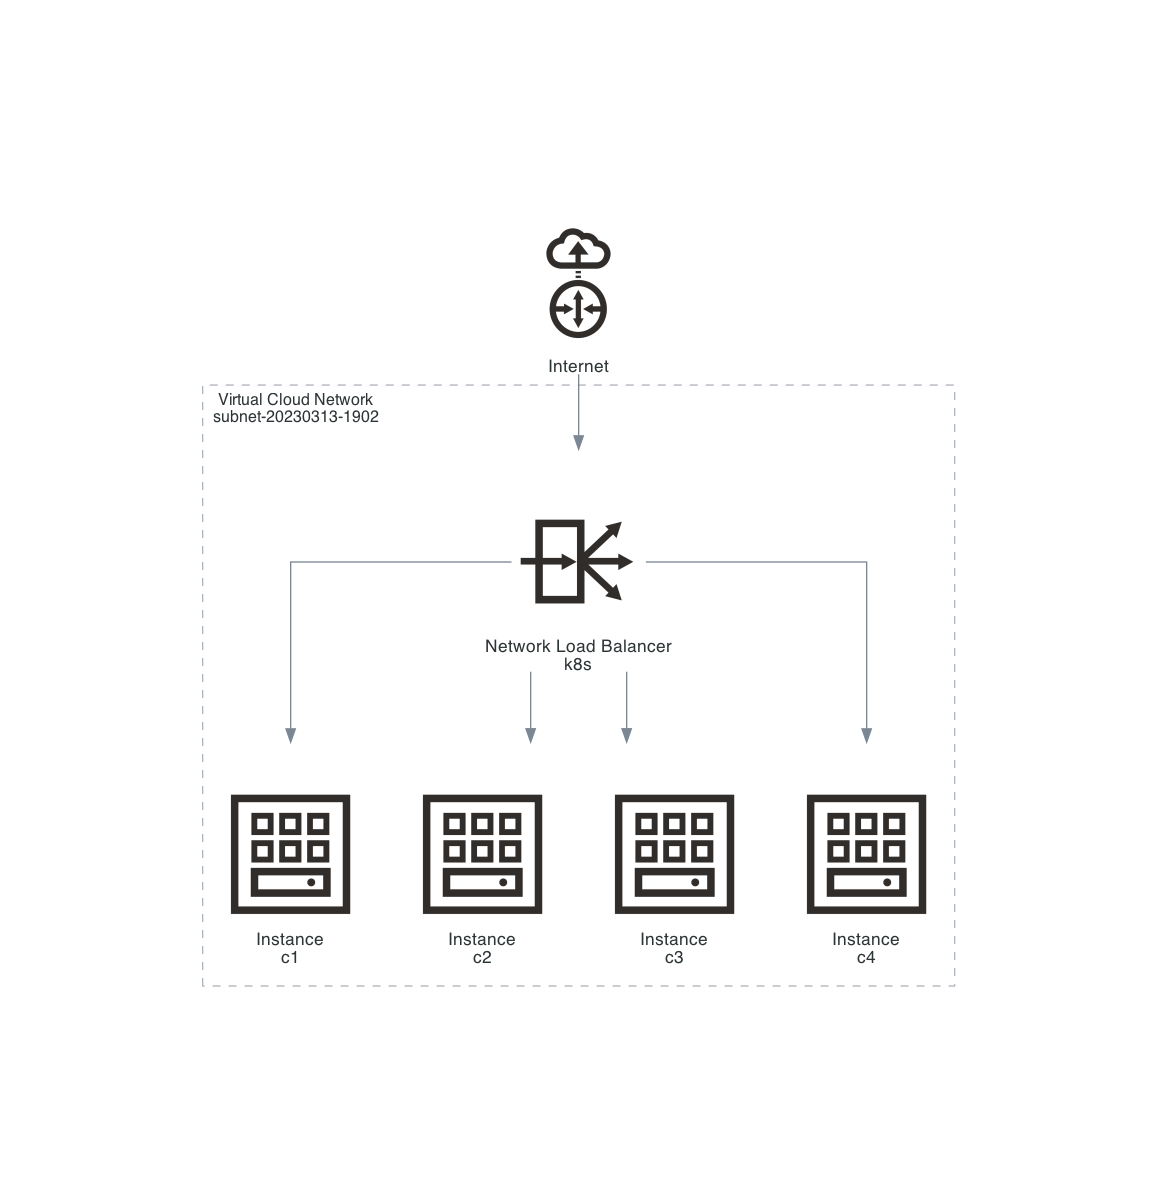
\includegraphics[width=\textwidth]{img/oci-infrastructure}
    \caption{Zaprojektowana infrastruktura}
    \label{fig:infrastructure}
\end{figure}

\subsection{Maszyny wirtualne}

Każdy węzeł klastra został uruchomiony na oddzielnej maszynie wirtualnej (ang. \emph{virtual machine, VM}).
Wszystkie węzły, w formie tabelki, przedstawiono na rysunku~\ref{fig:oci-compute-instances}.

\begin{figure}[H]
    \centering
    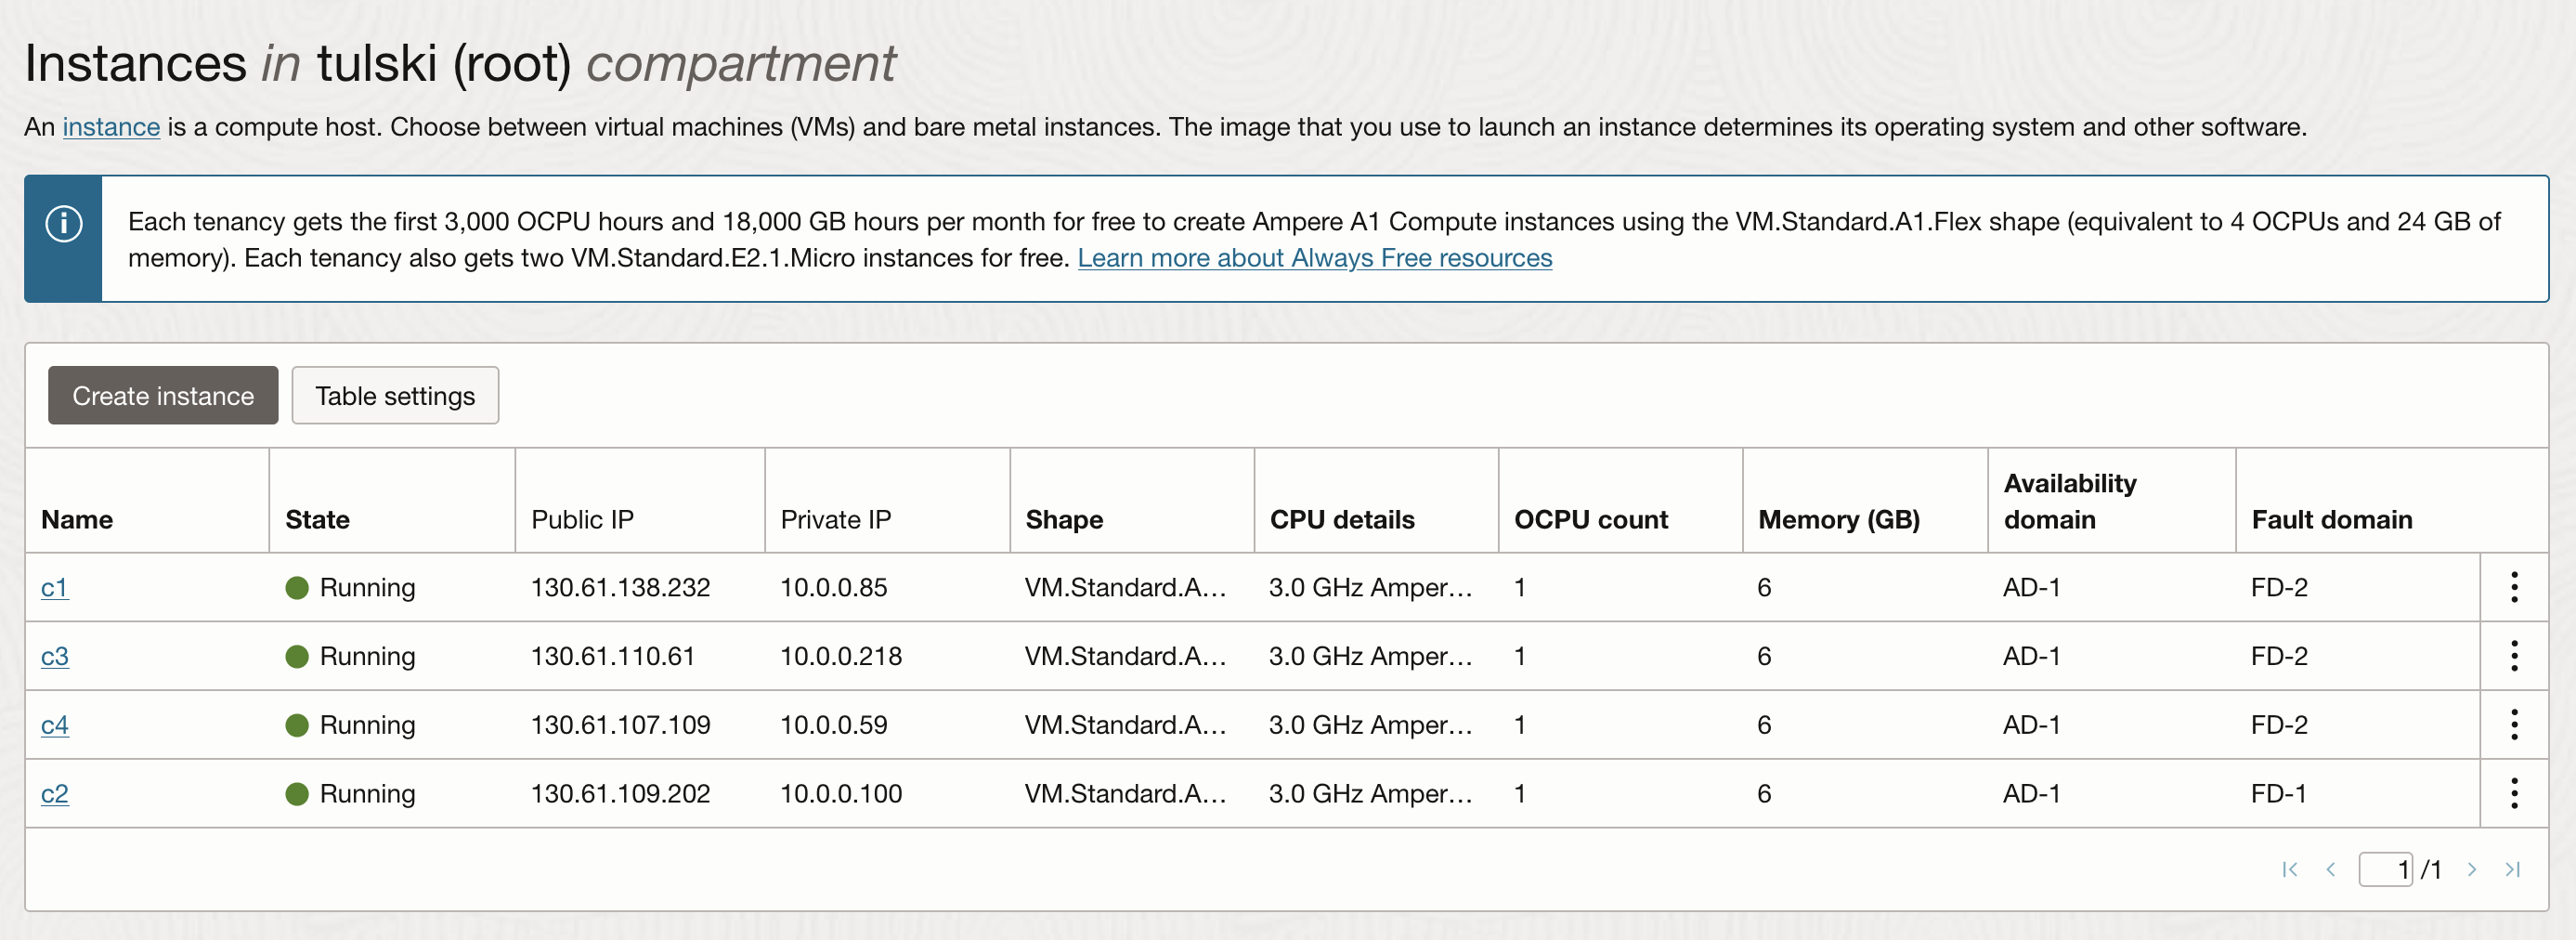
\includegraphics[width=\textwidth]{img/oci-compute-instances}
    \caption{Lista wszystkich maszyn wirtualnych}
    \label{fig:oci-compute-instances}
\end{figure}

\noindent Specyfikacja każdej z maszyn wirtualnych:
\begin{itemize}
    \item Kształt: VM.Standard.A1.Flex (Procesor Arm od Ampere)
    \item Liczba OCPU: 1
    \item Przepustowość sieci: 1 Gbps
    \item Pamięć RAM: 6 GB
    \item Obraz: Canonical Ubuntu 22.04 aarch64 2023.02.15-0
\end{itemize}

\noindent Szczegółową specyfikację jednej z maszyn wirtualnych przedstawiono na rysunku~\ref{fig:oci-instance-details}.

\begin{figure}[H]
    \centering
    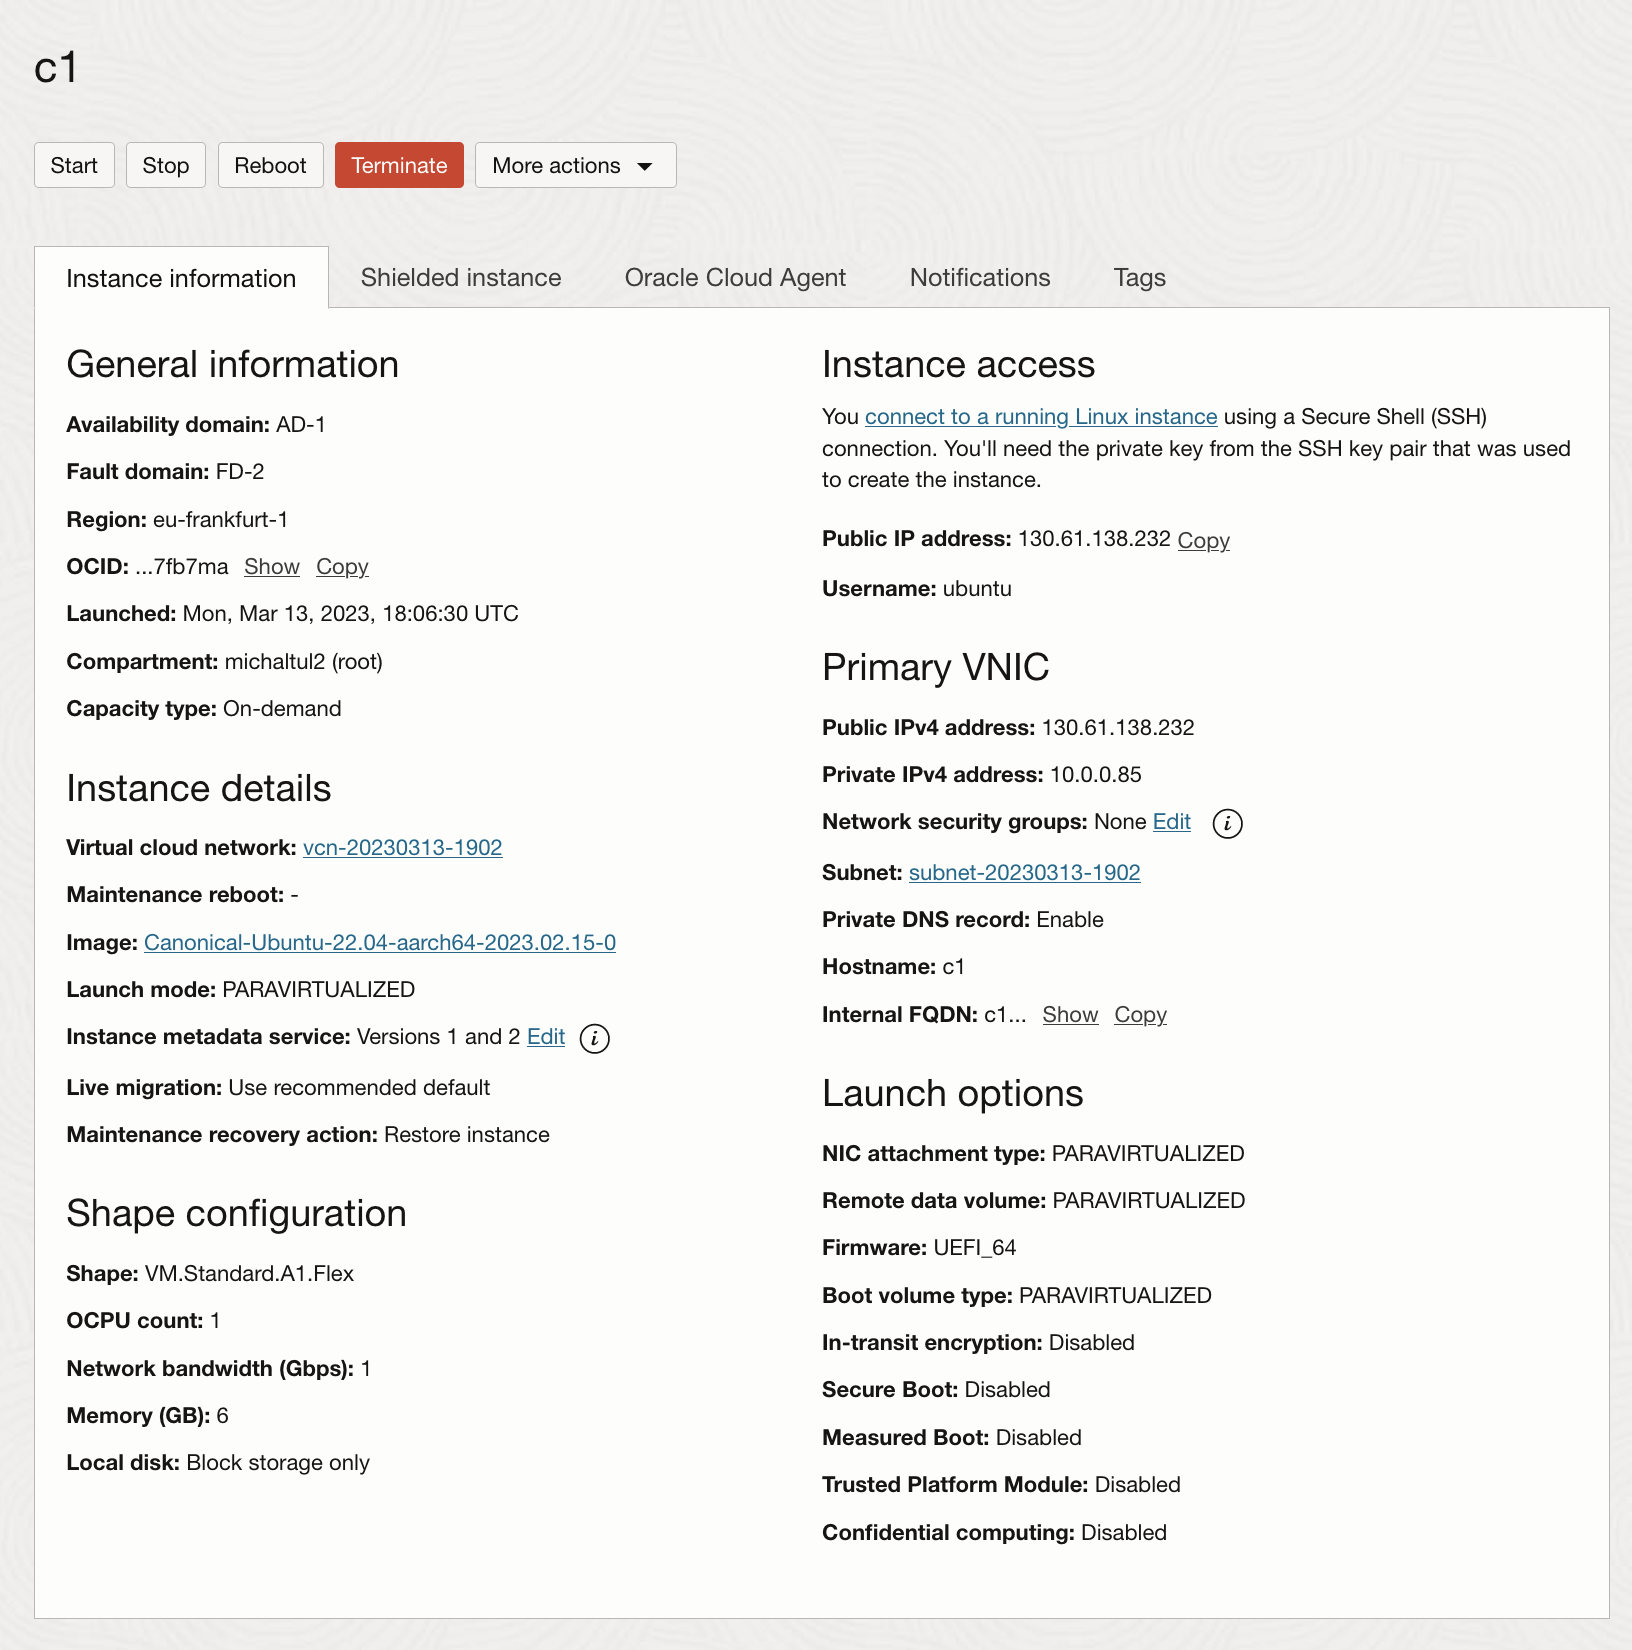
\includegraphics[width=\textwidth]{img/oci-instance-details}
    \caption{Specyfikacja maszyny wirtualnej c1}
    \label{fig:oci-instance-details}
\end{figure}

\subsection{Konfiguracja podsieci}

Wszystkie zasoby znajdują się w jednej wirtualnej podsieci (ang. \emph{virtual cloud network}, VCN) subnet-20230313-1902, która stanowi bezpieczne i izolowane środowisko sieciowe.
Informacje o podsieci przedstawiono na rysunku~\ref{fig:oci-subnet}.

\begin{figure}[H]
    \centering
    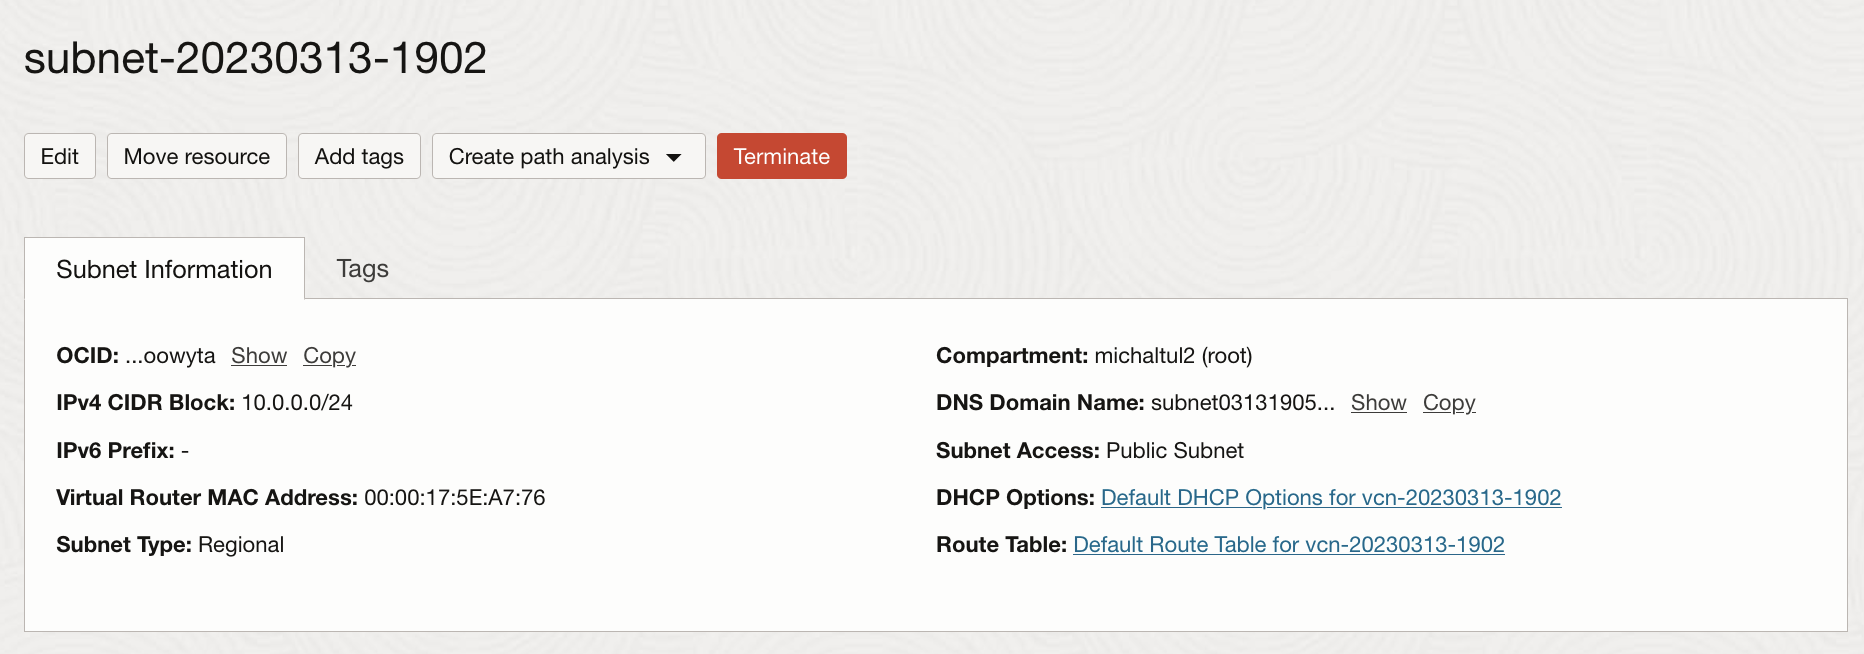
\includegraphics[width=\textwidth]{img/oci-subnet}
    \caption{Podsieć subnet-20230313-1902}
    \label{fig:oci-subnet}
\end{figure}

\noindent Domyślne reguły VCN\cite{oci-security-lists} pozwalają na:
\begin{enumerate}
    \item ruch TCP na porcie usługi SSH (22) z autoryzowanych adresów IP\@,
    \item ruch ICMP typu 3 o kodzie 4 (ang. \emph{Fragmentation Needed and Don't Fragment was Set}) z dowolnego adresu IP,
    \item ruch ICMP typu 3 z wszystkich hostów znajdujących się w danej podsieci,
    \item ruch wychodzący.
\end{enumerate}

\noindent Aby wykorzystać klaster jako platformę wdrożeniową dla aplikacji internetowych, konieczne jest dodanie dwóch dodatkowych reguł.

\begin{enumerate}
    \item Reguła pozwalająca na ruch TCP z dowolnego źródła na porty 80 i 443.
    \item Reguła pozwalająca na cały ruch z adresu IP administratora - wymagana do zdalnego zarządzania klastrem przez Kubernetes API (kubectl).
\end{enumerate}

\noindent Kompletna lista wszystkich reguł sieciowych dla stworzonej podsieci subnet-20230313-1902 została zaprezentowana na rysunku~\ref{fig:oci-subnet-ingress-rules}.

\begin{figure}[H]
    \centering
    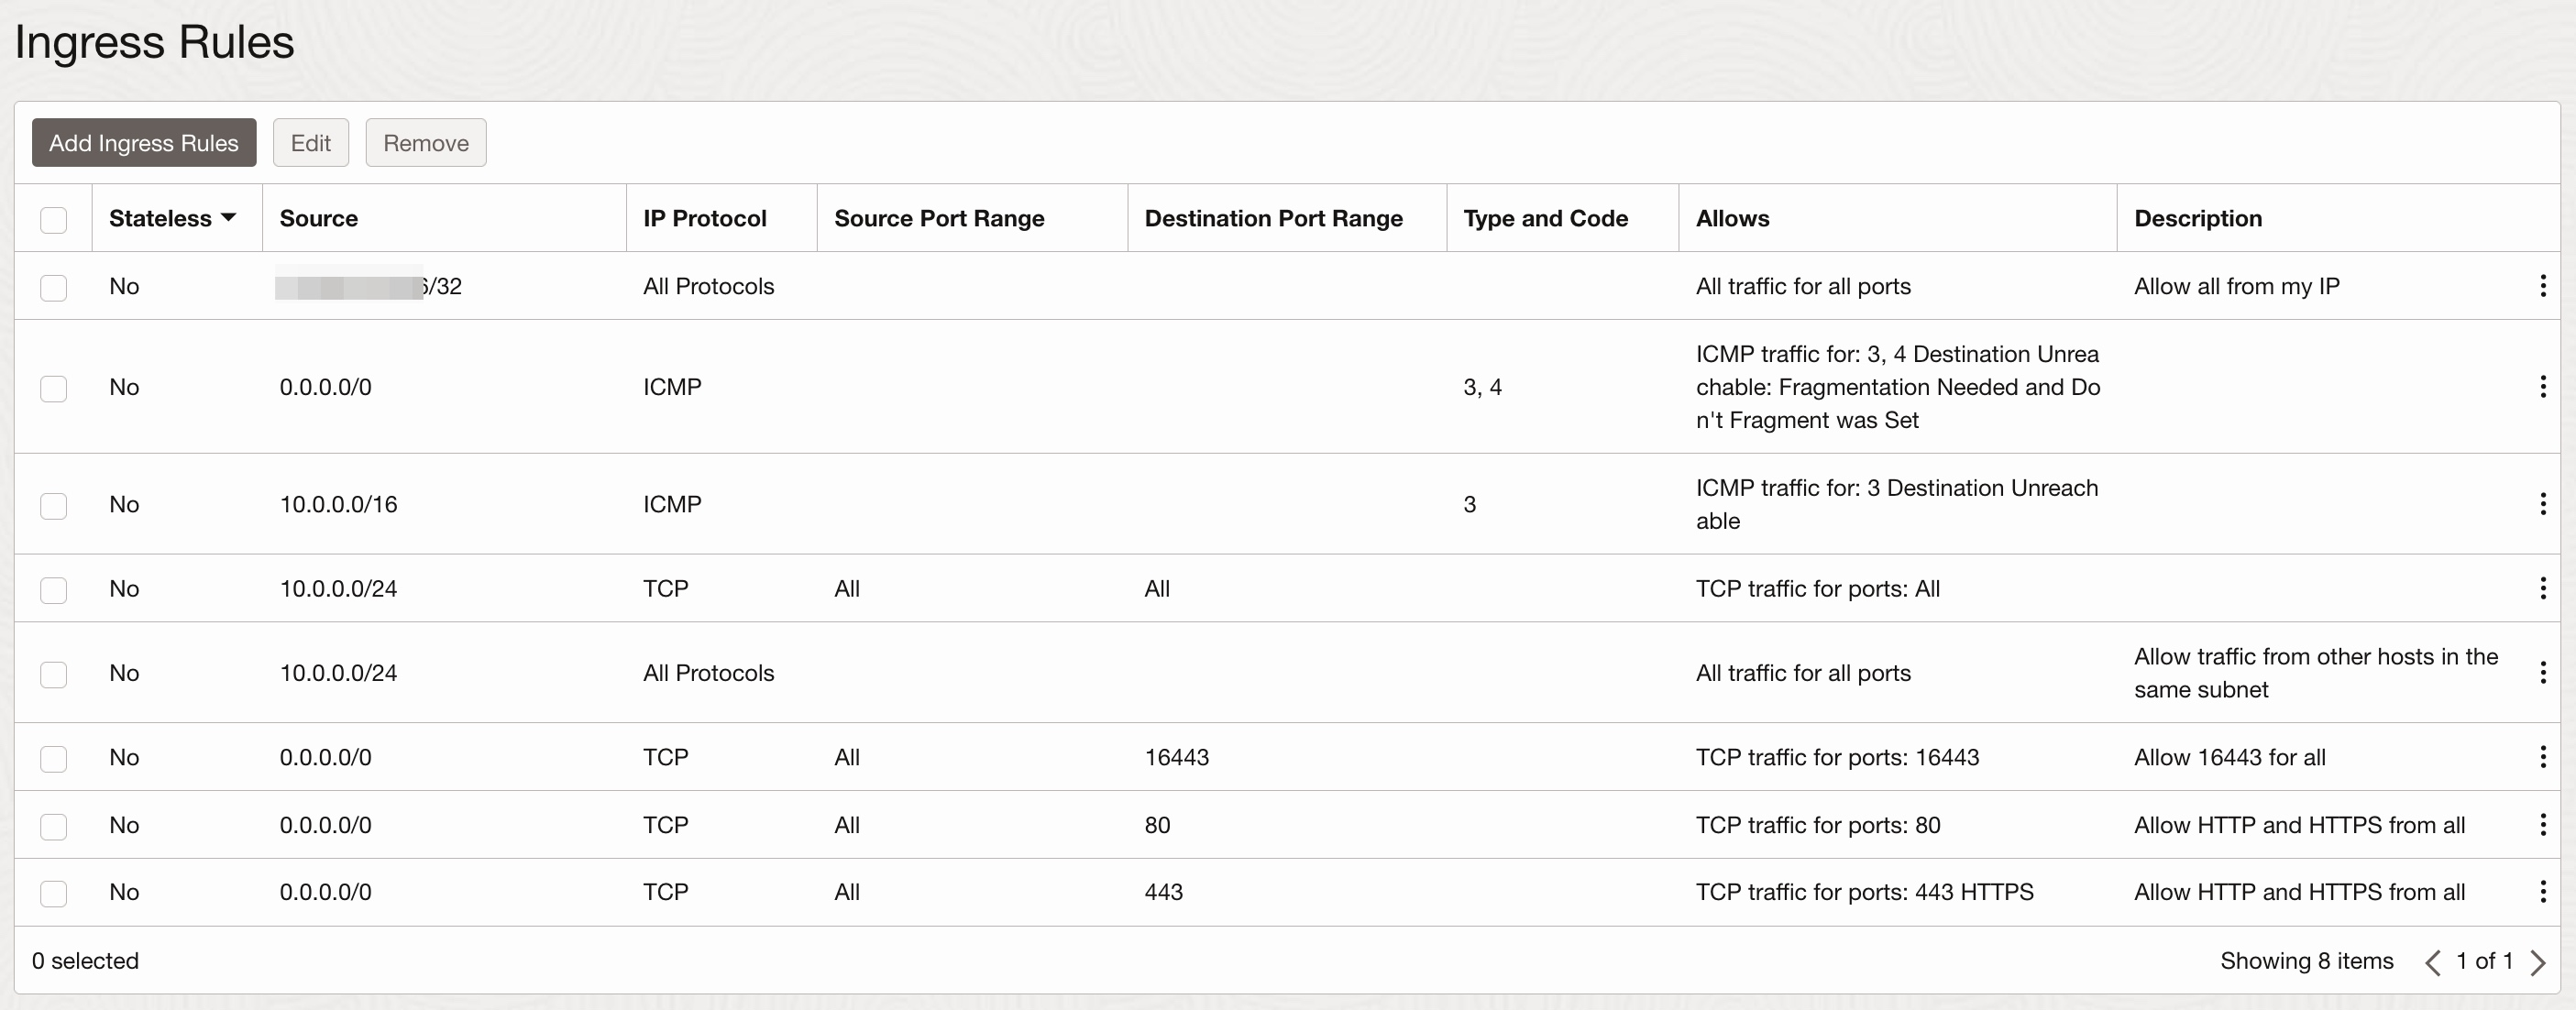
\includegraphics[width=\textwidth]{img/oci-subnet-ingress-rules}
    \caption{Reguły dla ruchu przychodzącego}
    \label{fig:oci-subnet-ingress-rules}
\end{figure}

Zmiany na poziome usług sieciowych OCI są niewystarczające, ponieważ ruch zostanie zablokowany przez domyślne reguły firewalla systemowego maszyn wirtualnych.
Aby osiągnąć oczekiwany rezultat konieczna jest modyfikacja pliku \texttt{/etc/iptables/rules.v4} na każdej z maszyn wirtualnych.

\noindent Należy dodać dwie reguły:

\begin{enumerate}
    \item Reguła zezwalająca na ruch wejściowy pochodzący z publicznego adresu IP administratora.\\
    \mintinline{text}{-I INPUT -s ADMIN_PUBLIC_IP/32 -j ACCEPT}
    \item Reguła pozwalająca na ruch przychodzący z dowolnego adresu w podsieci.\\
    \mintinline{text}{-I INPUT -s 10.0.0.0/24 -j ACCEPT}
\end{enumerate}

\noindent Dodatkowo, konieczne jest usunięcie wpisu, który blokuje wiadomości ICMP (ping):\\
\mintinline{text}{-A FORWARD -j REJECT --reject-with icmp-host-prohibited}

\subsection{Network Load Balancer}

Load Balancer (LB) to technologia, która, podobnie do reverse proxy, ma na celu kierowanie żądań użytkowników do odpowiednich serwerów.
Każdy LB implementuje pewien zestaw reguł i algorytmów, który równomiernie rozkładają ruch na wszystkie serwery w grupie mogące go obsłużyć, tak aby sprostować aktualnemu obciążeniowi.
Dzięki temu zapewnia pryncypium wysokiej dostępności (high availability), niezawodności i skalowalność systemu.
W związku z tym, że Load Balancer ciągle monitoruje aktywność węzłów, jest w stanie szybko wykryć ewentualną awarię i automatycznie przekierować ruch do pozostałych, sprawnych węzłów.
Prostą analogią dla Load Balancera jest policjant stojący na skrzyżowaniu.

Dodatkową zaletą LB jest uproszczenie konfiguracji DNS - wystarczy dodanie jednego rekord typu A z publicznym adresem IP wskazującym na LB\@.
Eliminuje to potrzebę tworzenia osobnych wpisów dla każdego węzła, co komplikowałoby konfigurację i utrudniałoby jej utrzymanie.

Z powodu zapewnienia wysokiej dostępności, równomiernego rozłożenia ruchu, skalowalności i uproszczeniu konfiguracji DNS, jak i wielu innych niewspomnianych korzyści, LB jest kluczowym elementem wielu rozbudowanych systemów.

Jednym z rodzajów Load Balancera jest Network Load Balancer (NLB), który działa na warstwie 3 i 4 modelu OSI wykorzystując protokoły TCP, UDP i ICMP\@.
NLB przekazuje pakiety do i z serwera nadrzędnego na podstawie informacji na poziomie IP, portu i protokołu bez sprawdzania pakietów.

Utworzony Network Load Balancer k8s znajduje się w wcześniej stworzonej podsieci subnet-20230313-1902.

\autoref{fig:oci-network-load-balancer-k8s} przedstawia informacje o wdrożonym NLB k8s.

\begin{figure}[H]
    \centering
    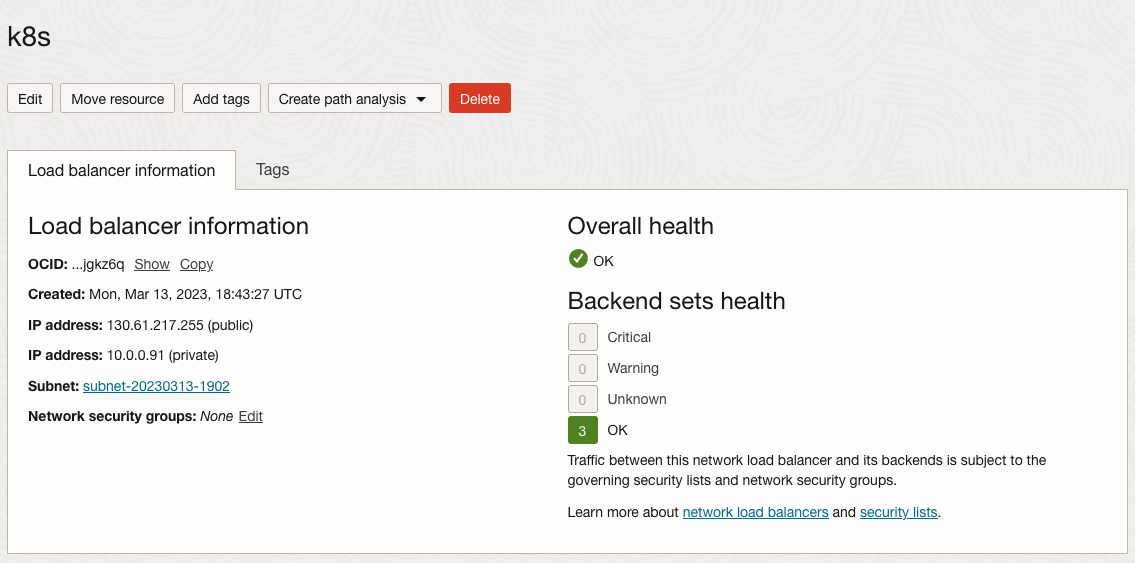
\includegraphics[width=\textwidth]{img/oci-network-load-balancer-k8s}
    \caption{Informacje o NLB k8s}
    \label{fig:oci-network-load-balancer-k8s}
\end{figure}

NLB k8s został skonfigurowany tak aby działał dla ruchu HTTP (port 80), HTTPS (port 443) oraz Kubernetes API (port 16443).
Dla każdego z rodzajów ruchu został utworzony Backend Set (zob. \autoref{fig:oci-network-load-balancer-k8s-backend-sets}) oraz Listener (zob. \autoref{fig:oci-network-load-balancer-k8s-listeners}).

\begin{figure}[H]
    \centering
    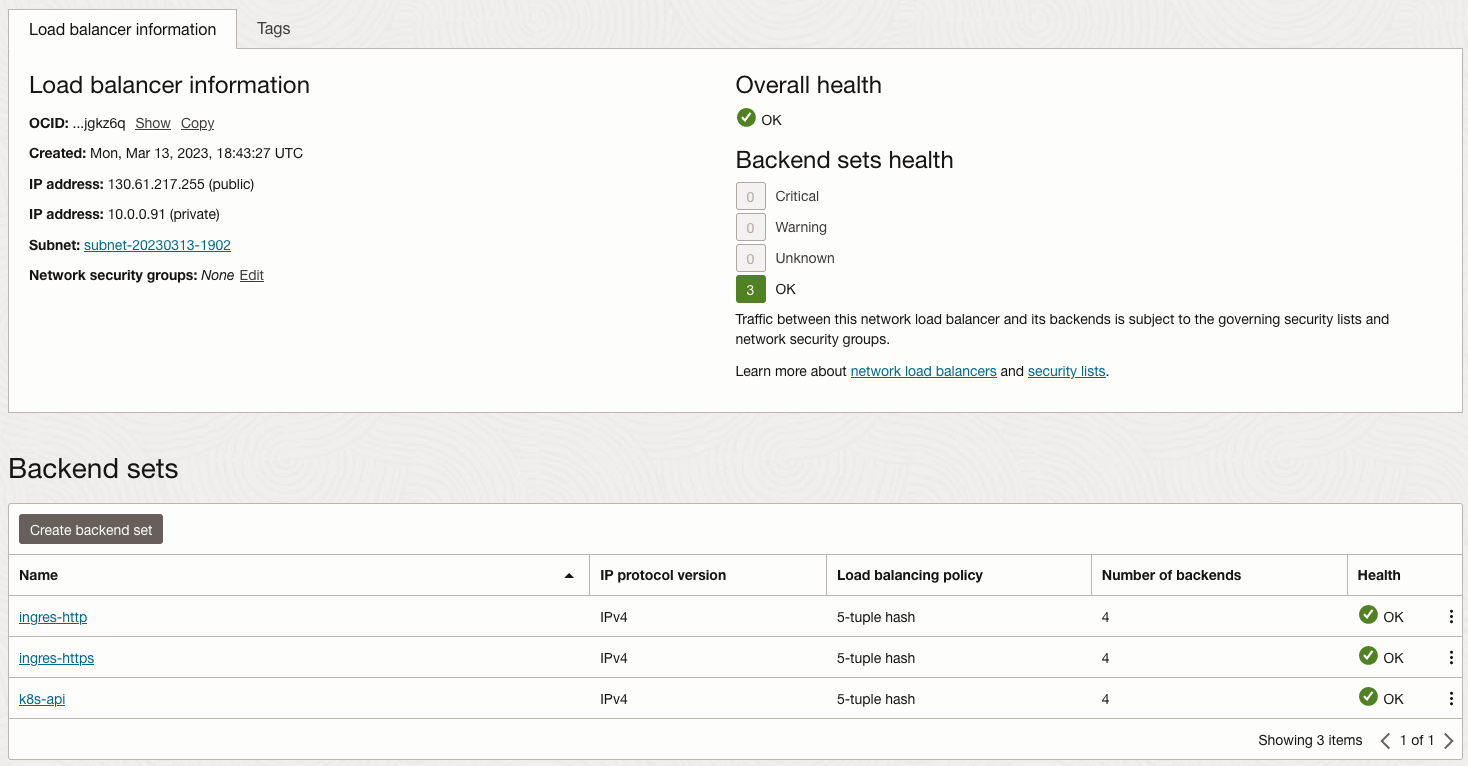
\includegraphics[width=\textwidth]{img/oci-network-load-balancer-k8s-backend-sets}
    \caption{Backend Sets stworzonego Network Load Balancera k8s}
    \label{fig:oci-network-load-balancer-k8s-backend-sets}
\end{figure}

\begin{figure}[H]
    \centering
    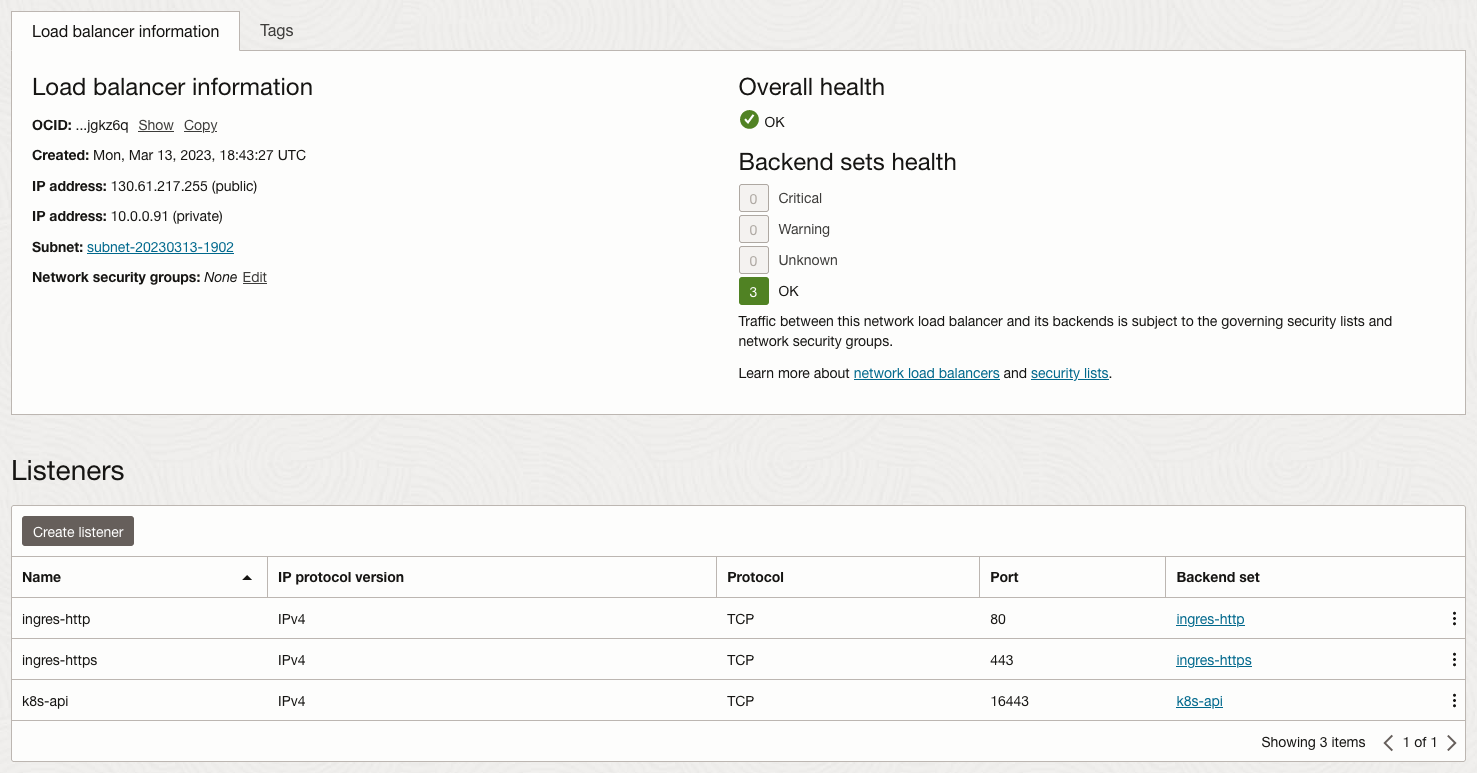
\includegraphics[width=\textwidth]{img/oci-network-load-balancer-k8s-listeners}
    \caption{Listeners stworzonego Network Load Balancera k8s}
    \label{fig:oci-network-load-balancer-k8s-listeners}
\end{figure}

Load Balancer regularnie monitoruje aktywność każdego węzła za pomocą zdefiniowanego testu Health Check.
Dla pierwszych dwóch Backend Sets - \texttt{ingress-http} (zob. \autoref{fig:oci-network-load-balancer-ingress-http-health-check}) oraz \texttt{ingress-https} (zob. \autoref{fig:oci-network-load-balancer-ingress-https-health-check})- test polega na wysłaniu zapytania z użyciem kolejno protokołu HTTP i HTTPS na ścieżkę \url{/}.
Oczekiwaną odpowiedzią serwera jest status 404.

\begin{multicols}{2}
    \begin{figure}[H]
        \centering
        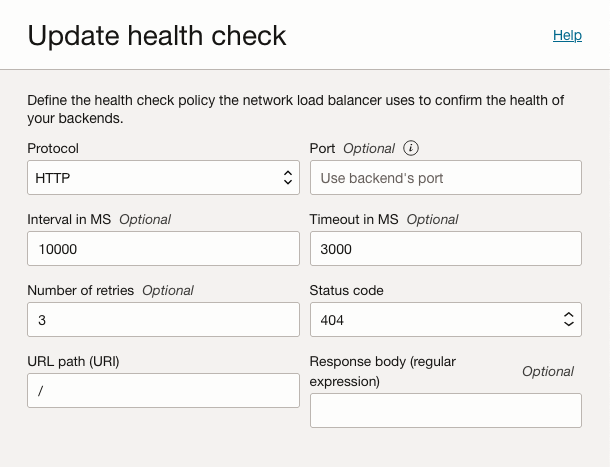
\includegraphics[width=0.5\textwidth]{img/oci-network-load-balancer-ingress-http-health-check}
        \caption{Health Check dla ingress-http}
        \label{fig:oci-network-load-balancer-ingress-http-health-check}
    \end{figure}
    \begin{figure}[H]
        \centering
        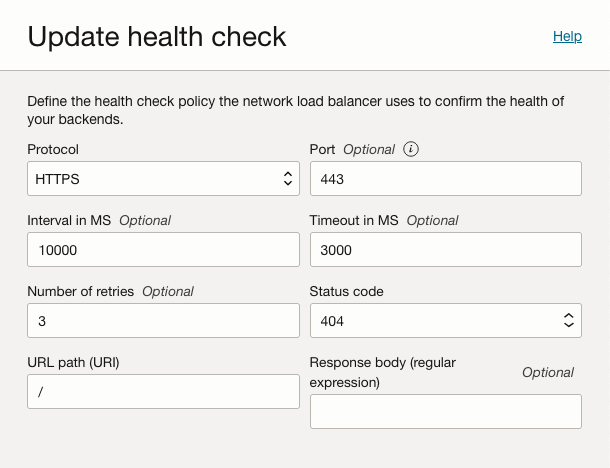
\includegraphics[width=0.5\textwidth]{img/oci-network-load-balancer-ingress-https-health-check}
        \caption{Health Check dla ingress-https}
        \label{fig:oci-network-load-balancer-ingress-https-health-check}
    \end{figure}
\end{multicols}

Ostatni Backend Set, czyli  k8s-api, polega na wysłaniu zapytania protokołem HTTPS na port 16443 do ścieżki \url{/healthz}, gdzie oczekiwaną odpowiedzią serwera jest status 200 (zob. \autoref{fig:oci-network-load-balancer-k8s-api-health-check}).
\begin{figure}[H]
    \centering
    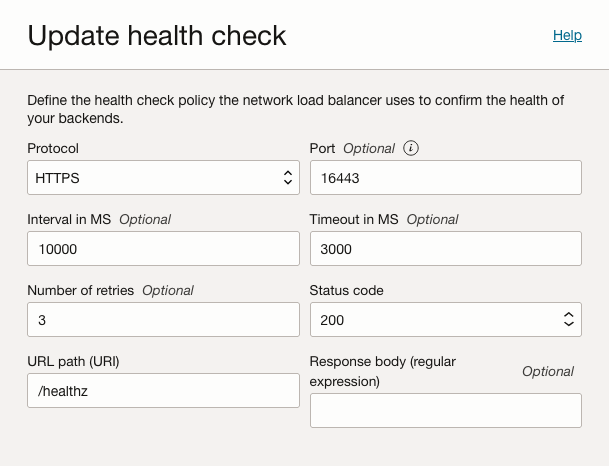
\includegraphics[width=0.7\textwidth]{img/oci-network-load-balancer-k8s-api-health-check}
    \caption{Health Check dla k8s-api}
    \label{fig:oci-network-load-balancer-k8s-api-health-check}
\end{figure}

\subsection{Instalacja Kubernetes}

Klaster wykorzystuje dystrybucję MicroK8s (zob. \autoref{subsec:microk8s}) w wersji 1.23.
Instalację MicroK8s przeprowadzono na każdej z maszyn wirtualnych poleceniem~\autoref{lst:microk8s-install}.

\begin{listing}[H]
    \begin{minted}{bash}
    apt update && \
        apt install docker.io -y && \
        snap install microk8s --classic --channel=1.23/stable
    \end{minted}
    \caption{Polecenie instalacyjne MicroK8s}
    \label{lst:microk8s-install}
\end{listing}

\subsection{Konfiguracja certyfikatów Kubernetes API}

Kubernetes API stanowi kluczowy element systemu z perspektywy cyberbezpieczeństwa.
Jednym z sposobów jego zabezpieczenia jest wymóg szyfrowanej komunikacji HTTPS, opartej na zweryfikowanym certyfikacie.
Domyślne generowane przez MicroK8s certyfikaty pozwalają na połączenia z lokalnych adresów IP (zwykle adresów LAN) oraz komunikację z adresami mDNS (komunikacja w obrębie klastra, z adresów takich jak kubernetes.default lub kubernetes.default.svc.cluster.local).
Aby umożliwić zdalne połączenie z Kubernetes API z internetu, niezbędna jest modyfikacja sekcji alt\_name pliku szablonu Certificate Signing Request (CSR) znajdującego się pod ścieżką \url{ /var/snap/microk8s/current/certs/csr.conf.template}.
Modyfikacja musi zostać wykonana na każdej z maszyn wirtualnych.

\noindent Modyfikacja polega na dodaniu do sekcji alt\_names:
\begin{enumerate}
    \item publicznego adresu IP maszyny wirtualnej,
    \item prywatnego adresu IP maszyny wirtualnej,
    \item publicznego adresu IP load balancera.
\end{enumerate}

\noindent\autoref{lst:domyslna-konfiguracja-alt-names} przedstawia domyślną, niezmienioną sekcję alt\_names.

\begin{listing}[H]
    \begin{minted}{text}
[ alt_names ]
DNS.1 = kubernetes
DNS.2 = kubernetes.default
DNS.3 = kubernetes.default.svc
DNS.4 = kubernetes.default.svc.cluster
DNS.5 = kubernetes.default.svc.cluster.local
IP.1 = 127.0.0.1
IP.2 = 10.152.183.1
    \end{minted}
    \caption{Domyślna sekcja alt\_names maszyny wirtualnej c1}
    \label{lst:domyslna-konfiguracja-alt-names}
\end{listing}

\noindent\autoref{lst:zmodyfikowana-konfiguracja-alt-names} przedstawia odpowiednio zmodyfikowaną sekcję alt\_names.

\begin{listing}[H]
    \begin{minted}{text}
[ alt_names ]
DNS.1 = kubernetes
DNS.2 = kubernetes.default
DNS.3 = kubernetes.default.svc
DNS.4 = kubernetes.default.svc.cluster
DNS.5 = kubernetes.default.svc.cluster.local
IP.1 = 127.0.0.1
IP.2 = 10.152.183.1
IP.100 = 130.61.138.232 # Publiczny adres IP maszyny wirtualnej
IP.110 = 10.0.0.85      # Prywanty adres IP maszyny wirtualnej
IP.120 = 130.61.217.255 # Publiczny adres IP load balancera
    \end{minted}
    \caption{Zmodyfikowana sekcja alt\_names na maszynie wirtualnej c1}
    \label{lst:zmodyfikowana-konfiguracja-alt-names}
\end{listing}

\noindent Po modyfikacji pliku konieczne jest uruchomienie polecenia odświeżającego certyfikaty MicroK8s (zob. \autoref{lst:polecenie-odswiezajace-certyfikaty}) i ponowne uruchomienie maszyny (reboot).

\begin{listing}[H]
    \begin{minted}{bash}
    sudo microk8s refresh-certs
    \end{minted}
    \caption{Polecenie odświeżające certyfikaty MicroK8s}
    \label{lst:polecenie-odswiezajace-certyfikaty}
\end{listing}

\subsection{Formowanie klastra Kubernetes}

\noindent Formowanie klastra w Kubernetes polega na zintegrowaniu węzłów uruchomionych na różnych maszynach wirtualnych, aby wspólnie tworzyły jednolity system.
Poniżej przedstawione są kroki niezbędne do uformowania klastra.

\begin{enumerate}
    \item Określ, która z maszyn wirtualnych będzie pełnić rolę głównego węzła (ang. \emph{master node}). To on będzie koordynować dodawanie kolejnych węzłów do klastra.
    \item Na wyznaczonym głównym węźle wykonaj polecenie \mintinline{bash}{microk8s add-node}.
          Wynikiem będzie polecenie do dołączenia do klastra mające postać:
    \begin{figure}[H]
        \begin{minted}{bash}
    microk8s join <vm_private_ip>:25000/<token>
        \end{minted}
        \label{fig:join-cluster-command}
    \end{figure}
    \item Wykonaj otrzymane w poprzednim kroku polecenie na każdej maszynie wirtualnej, która ma zostać częścią klastra, ale jeszcze w nim nie jest.
    \item Dla każdej kolejnej maszyny, która ma dołączyć do klastra, powtarzaj kroki 2 i 3.
\end{enumerate}

\end{document}
